\documentclass[11pt,a4paper]{article}

% USEPACKAGE LISTA
\usepackage[utf8]{inputenc}
\usepackage{amsmath}
\usepackage{mathtools}
\usepackage{marvosym} 
\usepackage{wrapfig}
\usepackage{hyperref}
\usepackage{float}
\usepackage{multicol}
\hypersetup{colorlinks,citecolor=black,filecolor=black,linkcolor=black,urlcolor=black}
\usepackage{pdfpages}
\usepackage{amsfonts}
\usepackage{amssymb}
\usepackage{fancyhdr}
\usepackage{graphicx}
\usepackage{t1enc}
\usepackage[magyar]{babel}
\usepackage{bm}
\usepackage{tikz, tcolorbox}
\usepackage{verbatim}
\usepackage{amsmath,esint}
\usepackage{setspace}

\usepackage{pgfplots}
\pgfplotsset{height = 10cm, width=15cm,compat=1.9}

\usepackage[left=2cm,right=2cm,top=2cm,bottom=2cm]{geometry}

\setlength{\parindent}{0pt}
\setlength{\parskip}{0em}
\pagestyle{fancy}
\fancyhf{}
\cfoot{\thepage. oldal}


% ITT KEZDŐDIK A DOKUMENTUM
\begin{document}
\begin{titlepage}
    \centering
  
    
\includegraphics[width=.8\textwidth]{bme_logo_nagy.jpg}
  
    \vspace{1em}
  
    {
      \large
      BUDAPESTI MŰSZAKI ÉS GAZDASÁGTUDOMÁNYI EGYETEM GÉPÉSZMÉRNÖKI KAR
    }
  
    \vspace{8em}
  
    {
      \Huge
      \textbf{Matematika szigorlati tételsor}
    }
  
    \vspace{10em}
  
    {
      \huge
      Matematika G1, G2, G3
  
      \vspace{.2em}
  
      \large
      (BMETE94BG01, BMETE94BG02, BMETE94BG03)
    }
  
    \vspace{4em}
  
    {
      \Large
      \textit{Készítette:}
  
      \vspace{.5em}
  
      \textbf{Kis Erhard, Kun László Ákos}
    }
  
    \vspace{20em}
  
    {
      \large
      BUDAPEST, 2023
    }
  \end{titlepage}
\begin{center}
   \Large \textbf{Matematika G1 szóbeli beugró kérdések - 2023}
\end{center}
\textbf{Halmazelmélet és komplex számok}
\begin{enumerate}
    \item Halmaz, metszet, unió, különbség
    \item Descartes-szorzat, hatványhalmaz
    \item Csoport, gyűrű, test
    \item Komplex számok algebrai, exponenciális, trigonometrikus alakja
    \item Komplex számok hatványozása
    \item Komplex számok gyökvonása
\end{enumerate}
\textbf{Numerikus sorozatok}
\begin{enumerate}
    \item Numerikus sorozat fogalma és határértéke
    \item Konvergens, divergens sorozat
    \item Nevezetes sorozatok
    \item Cauchy-sorozat
    \item Torlódási pont
\end{enumerate}
\textbf{Függvények, derivált}
\begin{enumerate}
    \item Függvény, értelmezési tartomány, értékkészlet
    \item Függvény határértéke
    \item Függvény folytonossága
    \item Inverz függvény
    \item Derivált
    \item Lokális szélsőérték definíciója és feltétele
    \item L'Hospital szabály
    \item Taylor-polinom
\end{enumerate}
\textbf{Középértéktételek és integrálás}
\begin{enumerate}
    \item Lagrange-féle középértéktétel
    \item Rolle-féle középérték tétel
    \item Cauchy-féle középérték tétel
    \item Riemann-integrálhatóság
    \item Newton-Leibniz-formula
    \item Improprius integrálok
\end{enumerate}
\textbf{Numerikus sorok}
\begin{enumerate}
    \item Numerikus sor fogalma
    \item Numerikus sor konvergenciája (feltételes is),
    \item Numerikus sor divergenciája
    \item Konvergenciatesztek
\end{enumerate}

\newpage
\textbf{Halmazelmélet és komplex számok:}

\begin{tcolorbox}[colback=green!5!white,colframe=green!60!black,title= 1. Halmaz{,} unió{,} metszet{,} különbség]
    \textbf{Halmaz:} Közös tulajdonságú elemek összessége.\\\\
    \textbf{Unió:} Két vagy több halmaz uniója mindazon elemek halmaza, amelyek legalább az egyik halmaznak elemei.
                $$A \cup  B = \{ x \in X\mid x \in A \vee  x \in B\}$$
    \textbf{Metszet:} Két vagy több halmaz metszete pontosan azoknak az elemeknek a halmaza, melyek mindegyik halmaznak elemei
                $$A \cap   B = \{ x \in X\mid x \in A \wedge x \in B\}$$
    \textbf{Különbség:} \(A\) és \(B\) halmaz különbsége az \(A\) halmaz mindazon elemeinek halmaza, amelyek a \(B\) halmaznak nem elemei
                $$A \setminus   B = \{ x \in X\mid x \in A \wedge x \ni B\}$$
    \begin{center}
        \fbox{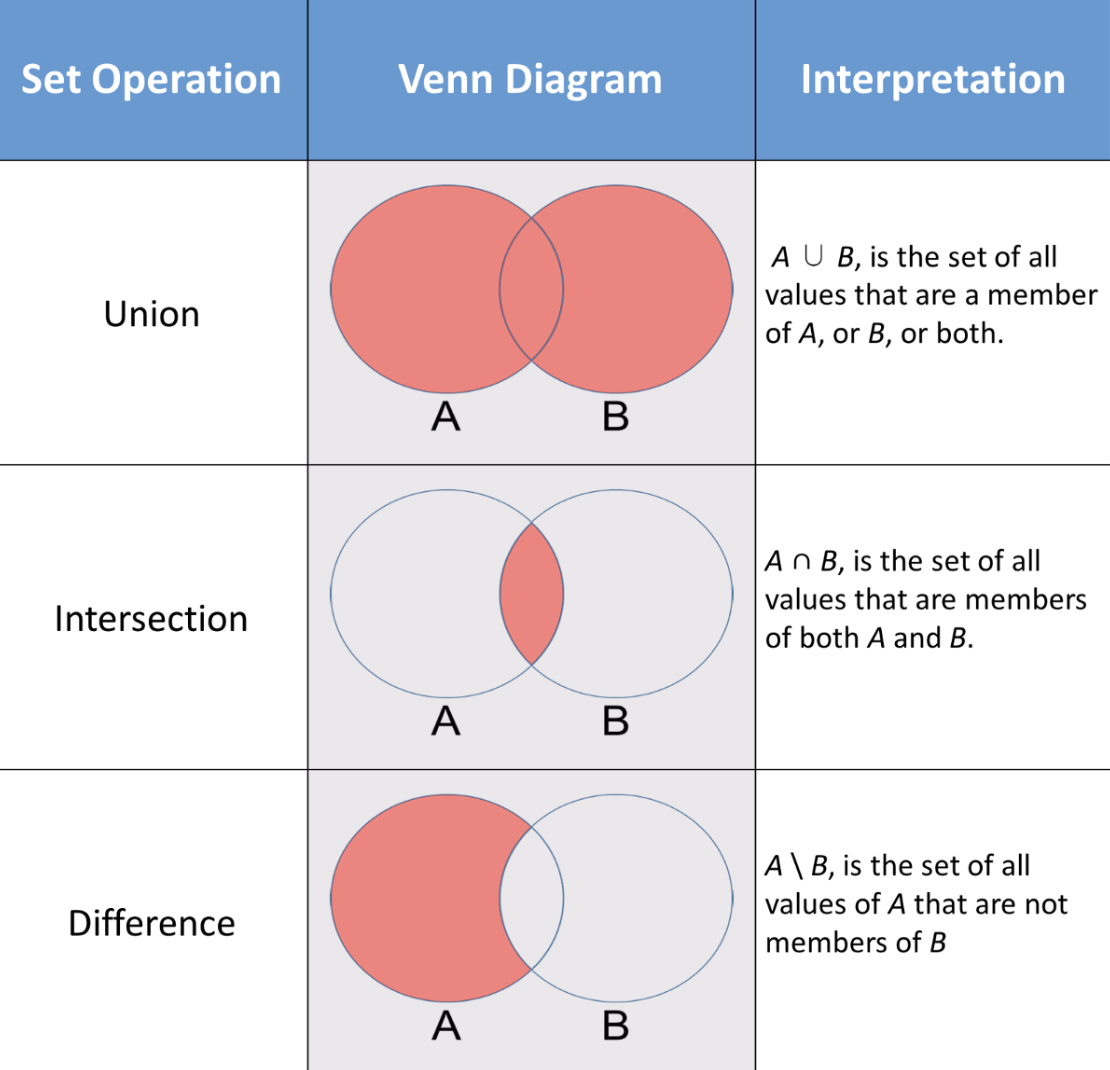
\includegraphics[scale = 0.5]{1.png}}
    \end{center}
\end{tcolorbox}

\begin{tcolorbox}[colback=green!5!white,colframe=green!60!black,title= 2. Descartes-szorzat{,} hatványhalmaz]
    Az A és B Halmazok Descartes-szorzatán az A és B Halmazok elemeiből alkotott összes rendezett elempárok halmazát értjük.
    $$A \times B := \{(a,b)\mid a \in A \wedge b \in B\}$$
    \textbf{Hatványhalmaz:} Egy halmaz összes részhalmazainak halmazát a Halmaz hatványhalmazának hívjuk.
\end{tcolorbox}

\begin{tcolorbox}[colback=green!5!white,colframe=green!60!black,title= 3. Csoport{,} gyűrű{,} test]
        \textbf{Félcsoport:} olyan halmaz, melyben a kétváltozós műveletek asszociatívak (pl. természetes számok esetén az összeadás)\\\\
        \textbf{Csoport:} Legyen \(G\neq 0\) és egy \(\circ \) művelet (szorzás). Ekkor \((G, \circ )\) csoport, ha teljesülnek az alábbiak:
        \begin{enumerate}
            \item \((a \circ b) \circ c = a \circ (b \circ c)\) minden \(a, b, c \in G\) esetén
            \item bármely \(e \in G\), hogy \(a \circ e = e \circ a = a\) minden \(a \in G\) esetén (létezik az egységelem, \(e\), amely asszociatív)
            \item minden \(a \in G\) esetén létezik \(a' \in G\), hogy \(a \circ a'=a' \circ a = e\) (létezik inverzelem)
        \end{enumerate}
        \textbf{Ábel-csoport:} olyan halmaz, melyben a kétváltozós műveletek asszociatívak és kommutatívak is ill. létezik a zérus elem és az inverz elem\\\\
        \textbf{Gyűrű:}
        Legyen \(R\neq 0\) és \(+, \circ \) két művelet. Ekkor \((R, +, \circ )\) gyűrű ha teljesülnek az alábbiak:
        \begin{enumerate}
            \item \((R, +)\) Ábel csoportot alkot (Ábel csoport = kommutatív csoport)
            \item A  művelet asszociatív (csoportosítható) \((a \circ b) \circ c = a \circ (b \circ c)\) minden \(a, b, c \in R\) esetén
            \item A \(\circ \) művelet disztributív \(+\)-ra nézve (összekapcsolható) \((a + b) \circ c = a \circ c + b \circ c\) minden \(a, b, c \in R\) esetén
        \end{enumerate}
        \textbf{Test:} 
        Legyen \(T \neq 0\) és \(+, \circ \) két művelet. Ekkor \((T, +, \circ)\) test ha teljesülnek az alábbiak:
        \begin{enumerate}
            \item (T, +) Ábel csoportot alkot
            \item A \(\circ\) művelet legyen asszociatív (csoportosítható) \((a \circ b) \circ c = a \circ (b \circ c)\) minden \(a, b, c \in R\) esetén
            \item A \(\circ\) művelet legyen disztributív azaz \((a + b) \circ c = a \circ c + b \circ c\) minden \(a, b, c \in R\) esetén
            \item Létezik \(e \in G\), hogy \(a \circ e = e \circ a = a\) minden \(a \in T\) esetén (létezik egységelem a második műveletre)
            \item A \(+\) műveletekhez tartozó egységelem kivételével bármely \(a \in G\) esetén létezik \(a' \in G\), hogy \(a \circ a' = a' \circ a = e\) (létezik az inverz elem, kivéve az első művelethez \((+)\) tartozó egységelem
            esetében)
        \end{enumerate}
\end{tcolorbox}

\begin{tcolorbox}[colback=green!5!white,colframe=green!60!black,title= 4. Komplex számok algebrai{,} trigonometrikus{,} exponenciális alakja]
    \begin{itemize}
        \item \textbf{Algebrai alak:} \(z = a + b\cdot i\) (\(z\) valós része \(a\), képzetes része pedig \(b\))
        \begin{itemize}
            \item \textbf{konjugált:} \(\overline{z} = a - b\cdot i\)
            \item \textbf{abszolút érték:} \(\left\lvert z \right\rvert  = \sqrt{a^2+b^2}\) (Pitagorasz-tételből), és mivel: \\ \(z \cdot \overline{z} = (a + b\cdot i)(a - b\cdot i) = a^2 -(b\cdot i)^2=a^2+b^2\), ezért \( \left\lvert z\right\rvert =\sqrt{z \cdot \overline{z} }  \)
        \end{itemize}
        \item \textbf{Trigonometrikus (polár) alak:} \(z = r(cos(\varphi ) + i \cdot sin(\varphi))\), mivel
        $$ cos(\varphi)=\frac{a}{r} $$
        $$ sin(\varphi)=\frac{b}{r} $$
        Tehát \(a = r\cdot cos(\varphi)\) és \(b = r\cdot sin(\varphi)\), innen már egyértelműen következik a trigonometrikus alak az algebraiból \(r\)-t kiemelve \((a = r\cdot cos(\varphi)\) és \(b\cdot i = r \cdot i\cdot sin(\varphi))\)
        \item \textbf{Exponenciális alak:} \(z = r \cdot e^{i\cdot \varphi}\) - ez csak egy szimbólum, rövidítés, ami megkönnyíti a
        számolást a komplex számokkal, lényegében a trigonometrikus alak kicsit rövidebben.
    \end{itemize}
\end{tcolorbox}

\begin{tcolorbox}[colback=green!5!white,colframe=green!60!black,title= 5. Komplex számok hatványozása]
    \textbf{de Moivre-képlet:} 
    $$z^n = [r(cos(\varphi)+i\cdot sin(\varphi))]^n=r^n(cos(n\varphi)+i\cdot sin(n\varphi))$$
    \textbf{Bizonyítás:} Teljes indukció használatával
    \begin{enumerate}
        \item \(n=1\)-re és \(n=2\)-re \textbf{igaz}
        \item indukciós feltétel: \(n = k\)
        \item Ekkor \(z^k= r^k(cos(k\varphi)+i\cdot sin(k\varphi))\)
        \item ha \(n = k + 1\), akkor:
    \end{enumerate}
    $$z^{k+1}=z^k\cdot k = r^k(cos(k\varphi)+i\cdot sin(k\varphi))\cdot r(cos(\varphi) +i\cdot sin(\varphi))$$
    $$=r^{k+1}[cos(k\varphi + \varphi)+ i\cdot sin(k\varphi + \varphi)] =$$
    $$r^{k+1}[cos((k+1)\varphi)+ i\cdot sin((k+1)\varphi)] $$\\
    és \(k+1\) az \(n\) volt, tehát a bizonyítás kész.

\end{tcolorbox}

\begin{tcolorbox}[colback=green!5!white,colframe=green!60!black,title= 6. Komplex számok gyökvonása]
$$z_1^n = z_2=r_1^n\cdot (cos(n\varphi_1)+i\cdot sin(n\varphi_1)) = r_2\cdot (cos(\varphi_2)+i\cdot sin(\varphi_2))$$  
$$z_1 = \sqrt[n]{z_2} $$  
\textbf{Két komplex szám akkor egyenlő, ha a hosszuk és argumentumuk is egyenlő:}
    \begin{itemize}
        \item \(r_1= \sqrt[n]{r_2}\) \hspace{61pt} (\textbf{hossz})
        \item \(n\cdot \varphi_1 = \varphi_2 + k\cdot 2\pi\) \hspace{10pt} (\textbf{argumentum}) \(\rightarrow\) forgásszög, periodicitás miatt \(p = 2\pi \)
        \item Így \(\varphi_1 = \frac{\varphi_2+k\cdot2\pi}{n} \hspace{30pt}\) \(k \in \{0, 1, 2, ... , n - 1\}\)
        \item Tehát: 
    \end{itemize}
    $$\sqrt[n]{z}= \sqrt[n]{r}(cos(\frac{\varphi+k\cdot2\pi}{n}) + i\cdot sin(\frac{\varphi+k\cdot2\pi}{n}))$$
    Az \(n\)-edik gyökvonás után olyan komplex számokat kapunk, amik egy szabályos sokszög
    (\(n\)-szög) csúcsai! Tehát n-edik gyökvonás esetén \(n\) db komplex szám a megoldás.
\end{tcolorbox}
\newpage

\textbf{Numerikus sorozatok:}

\begin{tcolorbox}[colback=green!5!white,colframe=green!60!black,title= 1. Numerikus sorozat határértéke]
Az \((a_n)\) sorozatot konvergens és határértéke az \(a \in R\) akkor és csak akkor, ha bármely \(\varepsilon > 0\) értékhez
létezik olyan \(N(\varepsilon)\) küszöbindex, hogy a sorozat \(N(\varepsilon)\)-nél nagyobb indexű elemei az az \(\varepsilon\) sugarú környezetében vannak.
Az \((a_n)\) sorozatot konvergens és határértéke az \(a \in R\) akkor és csak akkor, ha bármely \(\varepsilon > 0\) sugarú
környezetén kívül a sorozatnak csak véges sok eleme van.
\end{tcolorbox}

\begin{tcolorbox}[colback=green!5!white,colframe=green!60!black,title= 2. Konvergens{,} divergens sorozat]
    \begin{itemize}
        \item \textbf{Definíció:} Az \((a_n)\) konvergens, ha van olyan \(a \in R\) szám, hogy minden \(\varepsilon > 0\) valós szám esetén létezik \(N(\varepsilon)\) valós küszöbszám, hogy
    \end{itemize}
        $$\left\lvert a_n -a\right\rvert < \varepsilon,\hspace{5pt}ha\hspace{5pt}n > N(\varepsilon)$$
    \begin{itemize}
        \item Az \("a"\) számot az \((a_n)\) határértékének hívjuk, és a \(\lim_{n \to \infty} a_n = a\)  vagy az \(a_n \to a\), ha \(n \to \infty \) jelölést használjuk.
        \item Az \((a_n)\) divergens, ha nem konvergens.
    \end{itemize}
\textbf{Tételek:}
\begin{itemize}
    \item Konvergens sorozat korlátos.
    \item Monoton korlátos sorozat konvergens.
    \item van határértéke/torlódási pontjai \(\rightarrow\) nem biztos, hogy konvergens
    \item \textbf{Bolzano-Weierstrass-tétel:} minden korlátos sorozatnak van konvergens részsorozata.
\end{itemize}
\end{tcolorbox}

\begin{tcolorbox}[colback=green!5!white,colframe=green!60!black,title= 3. Nevezetes sorozatok]
    Olyan sorozatok, amelyek határértékét nem kell bizonyítani, csak felhasználni!\\\\
    \textbf{Bernoulli-féle egyenlőtlenség:} ha \(x \geq  -1\), akkor \((1+x)^n \geq 1 + n\cdot x\)
    \begin{enumerate}
        \item \(a^n \to 0\), ha \(\left\lvert a\right\rvert <1\)\\
        \(a^n \to 1\), ha \(a=1\)\\
        \(a^n \to +\infty\), ha \(a>1\)\\
        \(a^n\) divergens, ha \(a<-1\)
        \item \(\sqrt[n]{a} \to 1\), ha \(n \to \infty (a>0)\)
        \item \(a^n\cdot n^k \rightarrow 0\), nullsorozat, ha \(\left\lvert a\right\rvert <1 \) és \(k\) rögzített természetes szám
        \item \(\sqrt[n]{n} \to 1\), ha \(n \to \infty \hspace{5pt}(n\geq 2)\)
        \item \(\frac{a^n}{n!} \to 0 (a \in \mathbb{R} )\)
    \end{enumerate}
    \textbf{Legfontosabb:}
    $$(1+\frac{\alpha}{n})^n \to e^{\alpha}$$
\end{tcolorbox}

\begin{tcolorbox}[colback=green!5!white,colframe=green!60!black,title= 4. Cauchy sorozat]
        \textbf{Definíció:} Az \((a_n)\)-t Cauchy-sorozatnak nevezzük, ha minden \(\varepsilon > 0\) esetén \(\exists N(\varepsilon)\) küszöbindex, hogy: 
        \begin{center}
            \(\left\lvert a_n -a_m\right\rvert  < \varepsilon\), ha \(n,m > N(\varepsilon)\) \(\hspace{15pt}\) \((n,m \in N)\)
        \end{center}
        \textbf{Tétel:} Cauchy-féle konvergencia kritérium (szükséges és elégséges feltétel). Az \((a_n)\) akkor és csak akkor konvergens, ha Cauchy sorozat!
\end{tcolorbox}

\begin{tcolorbox}[colback=green!5!white,colframe=green!60!black,title= 5. Torlódási pont]
        \textbf{Definíció:} A \(h\) a \(H\) halmaz torlódási pontja, ha \(h\) bármely környezetében van \(H\)-nak \(h\)-tól
        különböző eleme. A \(t\) szám a sorozat torlódási pontja, ha \(t\) akármilyen kicsi környezete a sorozat végtelen sok
        elemét tartalmazza. Például: \((-1)^n\)
\end{tcolorbox}
\newpage

\textbf{Függvények, derivált:}

\begin{tcolorbox}[colback=green!5!white,colframe=green!60!black,title= 1. Függvények{,} értelmezési tartomány{,} értékkészlet]
        \textbf{Függvény:} ha az \(A\) (nemüres) halmaz minden egyes eleméhez hozzárendeljük a \(B\)
        (nemüres) halmaz pontosan egy elemét, akkor ezt a leképezést függvénynek nevezzük.
        $$f:A \to B$$
        \textbf{Értelmezési tartomány:} azon elemek halmaza, melyekhez a függvény hozzárendel
        egy-egy elemet a B halmazból, jelen esetben ez az A halmaz.
        $$D_f = A$$
        \textbf{Értékkészlet:} A képhalmaz, azaz a \(B\) halmaz azon elemei, melyeket az \(f\) függvény
        ténylegesen hozzárendel az \(A\) valamelyik eleméhez. Az értékkészlet tehát része a képhalmaznak:
        $$R_f \subset B$$
\end{tcolorbox}

\begin{tcolorbox}[colback=green!5!white,colframe=green!60!black,title= 2. Függvény határérték]
Azt mondjuk, hogy az \(f\) függvény határértéke az \("a"\) pontban \(A\), ha minden \(\varepsilon > 0\) számhoz
létezik olyan \(\delta(\varepsilon)  > 0\), hogy ha \(0 < \left\lvert x-a \right\rvert  < \delta(\varepsilon)\), akkor \(|f(x) - A| < \varepsilon\).\\
/Ez a Cauchy-féle definíció/\\
\begin{center}
    \(|x - a| < \delta(\varepsilon)\) azt jelenti, hogy:
\end{center}
    $$- \delta(\varepsilon) < x - a < \delta(\varepsilon) \hspace{10pt} /+a$$
    $$a - \delta(\varepsilon) < x < a + \delta(\varepsilon)$$

\textbf{Szemléletesesen:} azt jelenti, hogy a függvényértékek \((f(x)-ek)\) tetszőlegesen megközelítik az
A számot, ha az \(\varepsilon\) értékek elég közel kerülnek \(a\)-hoz. Az \(f\) függvénynek az \("a"\) pontban acsa (akkor és csak akkor) van határértéke, ha van bal- és
jobboldali határértéke és ez a kettő megegyezik!
\begin{itemize}
    \item \textbf{Határérték a végtelenben:}
    \begin{itemize}
        \item Az \(f\) függvény határértéke \(+\infty\)-ben \(A\), ha minden \(\varepsilon > 0\) esetén van olyan \(N(\varepsilon)\), hogy
    \(|f(x) - A| < \varepsilon\), ha \(x > N(\varepsilon)\).
        \item Az \(f\) függvény határértéke \(-\infty\)-ben \(A\), ha minden \(\varepsilon > 0\) esetén van olyan \(N(\varepsilon)\), hogy
    \(|f(x) - A| < \varepsilon\), ha \(x < N(\varepsilon)\).
    \end{itemize}
    \item \textbf{A végtelen, mint határérték:}
    \begin{itemize}
        \item Az \(f\) függvény határértéke \(a\)-ban \(+ \infty\), ha bármely \(N > 0\) esetén van olyan \(\delta(N)\), hogy \(f(x) > N\), ha \(0 < |x - a| < \delta(N)\).
        \item Az \(f\) függvény határértéke \(a\)-ban \(- \infty\), ha bármely \(N > 0\) esetén van olyan \(\delta(N)\), hogy \(f(x) < N\), ha \(0 < |x - a| < \delta(N)\).
    \end{itemize}
\end{itemize}
\end{tcolorbox}

\begin{tcolorbox}[colback=green!5!white,colframe=green!60!black,title= 3. Függvény folytonosság]
    Az \(f\) függvény az értelmezési tartományának \("a"\) pontjában folytonos, ha ebben a pontban
létezik határértéke és ez egyenlő az adott pontbeli helyettesítési értékkel, azaz ha
$$\lim_{x \to a} f(x) = f(a) $$
    \begin{itemize}
        \item \textbf{Definíció:} Az \(f\) függvényt folytonosnak nevezzük az \(a \in D_f\) pontban, ha bármely \(\varepsilon > 0\)
        esetén van olyan \(\delta(\varepsilon) > 0\) szám, hogy ha \(|x - a| < \delta(\varepsilon)\), akkor \(|f(x) - f(a)| < \varepsilon\).
    \end{itemize}
    Az \(f\) függvény egy intervallumon egyenletesen folytonos, ha bármely \(\varepsilon > 0\) számhoz van
    olyan \(\delta > 0\) szám, hogy \(f\) értelmezési tartományának bármely \(x_1\), \(x_2\) elemére, amelyek
    távolsága egymástól kisebb \(\delta\)-nál, fennáll az alábbi egyenlőtlenség.
    $$|f(x_1) - f(x_2)| < \varepsilon$$
    \begin{itemize}
        \item \textbf{Tétel:} Az \(f\) függvény pontosan akkor folytonos értelmezési tartományának \("a"\) pontjában, ha
        ott balról és jobbról is folytonos.
        \item \textbf{Definíció:} Az \(f\) függvény folytonos az \( ] a, b [ \)-on, ha folytonos \(]a, b[ \) minden pontjában.
        Az f függvény folytonos az \([a, b]\)-on, ha folytonos \(]a, b[\)-on és \(a\)-ban balról, \(b\)-ben
        jobbról folytonos.
    \end{itemize}
    \textbf{A folytonosság néhány nevezetes következménye:}\\
        Ha \(f\) folytonos egy zárt intervallumon, akkor ott egyenletesen folytonos.\\\\
        \textbf{Bolzano-tétel:} ha a függvény a zárt intervallumon folytonos, és az intervallum két
        végpontjában az értékei különböző előjelűek, akkor az intervallum belsejében van
        zérushelye. Másképp: felvesz minden \(f(a)\) és \(f(b)\) közé eső értéket egy folytonos függvény egy zárt intervallumon.\\\\
        \textbf{Weierstrass-tétel:} Zárt intervallumon folytonos függvény felveszi a minimumát és a
        maximumát is függvényértékként; továbbá minden olyan értéket, ami a legnagyobb és
        legkisebb érték közé esik.

\end{tcolorbox}

\begin{tcolorbox}[colback=green!5!white,colframe=green!60!black,title= 4. Inverz függvény]
Ha az \(f:X \to Y\) függvénynél a leképezés irányát megfordítjuk, vagyis az \(Y\) halmaz elemeit
képezzük le az \(X\) halmaz elemeire, akkor ez a fordított leképezés általában nem függvény, mert nem biztos, hogy egy \(y \in Y\) elemnek egyetlen \(x \in X\) elem felel meg. Ezért fontos az, hogy f bijektív, azaz kölcsönösen egyértelmű legyen, mert ekkor az \(f-1\) -gyel jelölt fordított leképezés is már függvény lesz.    
    \begin{itemize}
        \item \textbf{Definíció:} Ha az \(f: X \to Y\) függvény kölcsönösen egyértelmű, akkor az \(f^{-1} = Y \to X\)
        függvényt \(f\) inverz függvényének nevezzük. Ekkor igaz az alábbi összefüggés:
    \end{itemize}
    $$f^{-1}(f(x)) = f(f^{-1}(x)) = x$$
\end{tcolorbox}

\begin{tcolorbox}[colback=green!5!white,colframe=green!60!black,title= 5. Derivált]
Ha létezik és véges az alábbi differenciálhányados határértéke:\\
$$Lim_{x\to a}\frac{f(x)-f(a)}{x-a}$$ \\
akkor azt az \(f\) függvény deriváltjának vagy \("a"\) pontbeli differenciálhányadosának nevezzük.\\ 
\textbf{Jelölés:} $$\frac{d f(a)}{d x} = f'(a)$$
\end{tcolorbox}

\begin{tcolorbox}[colback=green!5!white,colframe=green!60!black,title= 6. Lokális szélsőérték definíciója és feltétele]
Legyen \(f : I \subset  R \to R\); \(a\subset  I\)\\
    Azt mondjuk, hogy \(f\) függvénynek a pontban lokális maximuma van, ha létezik \(\delta > 0\), hogy:
    $$f(x) \leq  f(a) (\forall  x \in K)$$
    Azt mondjuk, hogy \(f\) függvénynek a pontban lokális minimuma van, ha létezik \(\delta > 0\), hogy:
    $$f(x) \geq  f(a) (\forall  x \in K)$$
    \textbf{Szükséges feltétel:}\\
    Ha \(f : I \subset  R \to R\) differenciálható függvény és \(f\)-nek  \(\alpha \in int.\hspace{5pt}I-ben\) (\(I\) belseje) szélsőértéke van, akkor\(f'(\alpha)=0\)\\\\
    \textbf{Elégséges feltétel:}\\
    Ha \(f : I \subset  R \to R\) differenciálható függvény és \(\alpha \in int. \hspace{5pt}I\) továbbá létezik \(r > 0\), és teljesül az alábbi
feltétel, akkor \(f\)-nek \(\alpha\)-ban lokális minimuma van.\\
$$f'(x) \leq 0 \to x\in](\alpha -r); \alpha[$$
$$f'(x) \geq 0 \to x\in]\alpha; (\alpha + r)[$$
    Ha \(f : I \subset  R \to R\) differenciálható függvény és \(\alpha \in int. \hspace{5pt}I\) továbbá létezik \(r > 0\), és teljesül az alábbi
feltétel, akkor \(f\)-nek \(\alpha\)-ban lokális maximuma van.
$$f'(x) \geq 0 \to x\in](\alpha -r); \alpha[$$
$$f'(x) \leq 0 \to x\in]\alpha; (\alpha + r)[$$

\end{tcolorbox}

\begin{tcolorbox}[colback=green!5!white,colframe=green!60!black,title= 7. L'Hôpital szabály]
    Legyen \(f\) és \(g\) differenciálható függvények az \(\alpha\) pont egy környezetében, továbbá:
    \begin{center}
        \(Lim_{x \to \alpha} f(x)=Lim_{x \to \alpha} g(x)=0\) \hspace{10pt} vagy \hspace{10pt} \(\left\lvert Lim_{x \to \alpha} f(x) \right\rvert = \left\lvert Lim_{x \to \alpha} g(x) \right\rvert = \infty  \)\\
        \(\alpha \in \{0; \pm \infty \}\)
    \end{center}
    Ekkor: 
    $$\frac{Lim_{x \to \alpha} f'(x)}{Lim_{x \to \alpha} g'(x)} = \frac{Lim_{x \to \alpha} f(x)}{Lim_{x \to \alpha} f(x)} $$
\end{tcolorbox}
\newpage
\textbf{Középérték tételek és Integrálás:}

\begin{tcolorbox}[colback=green!5!white,colframe=green!60!black,title= 1. Lagrange középérték tétel]
    Legyen \(f : I \subset R \to R\) folytonos \([a; b]\) intervallumon és differenciálható \(]a; b[\) intervallumon. Ekkor
létezik olyan \(\delta \in ]a; b[\) hogy:
$$f'(\delta) = \frac{f(b)-f(a)}{b-a}$$
\end{tcolorbox}

\begin{tcolorbox}[colback=green!5!white,colframe=green!60!black,title= 2. Rolle középérték tétel]
    Legyen \(f\) folytonos \([a; b]\) intervallumon és differenciálható \(]a; b[\) intervallumon, továbbá \(f(a) = f(b) = 0\)
Ekkor létezik \( \xi \in ]a; b[\) melyre teljesül, hogy:
$$f'(\xi) = 0$$
\end{tcolorbox}

\begin{tcolorbox}[colback=green!5!white,colframe=green!60!black,title= 3. Cauchy középérték tétel]
    Legyen \(f\) és \(g\) függvények folytonosak \([a; b]\) intervallumon és differenciálhatóak \(]a; b[\) intervallumon,
valamint tegyük fel, hogy \(g'(x) \neq 0\) bármely \(x \in ]a; b[\) esetén. Ekkor létezik olyan \(\delta \in]a; b[\) hogy:
$$\frac{f(b)-f(a)}{g(b)-g(a)} = \frac{f'(\delta)}{g'(\delta)}$$
\end{tcolorbox}

\begin{tcolorbox}[colback=green!5!white,colframe=green!60!black,title= 4. Riemann-Integrálhatóság]
    Az \(f\) függvény Riemann-integrálható \([a; b]\) intervallumon, ha a Darboux-féle alsó- és felső-integrálja
megegyezik. Ezt a közös értéket az \(f\) függvény Riemann-integráljának nevezzük.
\end{tcolorbox}

\begin{tcolorbox}[colback=green!5!white,colframe=green!60!black,title= 5. Newton-Leibniz formula]
    Legyen \(f\) függvény Riemann-integrálható \([a; b]\) intervallumon és \(F : [a; b] \to \mathbb{R} \) olyan primitív függvény,
hogy \(F\) folytonos \([a; b]\) intervallumon, \(F\) differenciálható \(]a; b[\) intervallumon és \(F'(x) = f(x)\) bármely
\(x \in ]a; b[\) Ekkor:
$$\int_{a}^{b} f = F(b)-F(a) $$
\end{tcolorbox}

\begin{tcolorbox}[colback=green!5!white,colframe=green!60!black,title= 6. Improprius integrál]
    Legyen \((a; b) \in \mathbb{R}_b \) és \((a < b)\) valamint
    \begin{enumerate}
        \item minden \([x; y] \subset  ]a; b[\) esetén \(f\) Riemann-int. \([x; y]\) intervallumon és \((x; y) \subset \mathbb{R}\)
        \item létezik olyan \(c \in \mathbb{R}  (a < c < b)\), hogy az alábbi határértékek léteznek és végesek:
    \end{enumerate}
    \begin{center}
        \(Lim_{x \to \alpha }\int_{x}^{c} f(t) \,dt\) \(\hspace{15pt}\) és \(\hspace{15pt}\) \(Lim_{y \to b }\int_{c}^{y} f(t) \,dt\)
    \end{center}
    Ekkor az \(I:= Lim_{x \to \alpha }\int_{x}^{c} f(t) \,dt +  Lim_{y \to b }\int_{c}^{y} f(t) \,dt \) összeget az \(f\) függvény improprius integráljának nevezzük \(]a; b[\) intervallumon és \(\int_{a}^{b} f(b) \,dt \) jelöljük.\\\\
    Azt is mondjuk, hogy az \(f\) függvény improprius Riemann-integrálja az \(]a; b[\) intervallumon konvergens.
Ha az 1. feltétel teljesül, de a 2. feltétel nem, akkor az \(f\) függvény improprius Riemann-integrálja
divergens.
\end{tcolorbox}

\newpage
\textbf{Numerikus sorok:}

\begin{tcolorbox}[colback=green!5!white,colframe=green!60!black,title= 1. Numerikus sor fogalma]
    Az \(a_n\) numerikus sorozat tagjaiból képzett végtelen összeget numerikus sornak nevezzük. Jelölése:
    $$\sum_{n = 1}^{\infty} a_n $$
\end{tcolorbox}

\begin{tcolorbox}[colback=green!5!white,colframe=green!60!black,title= 2. Numerikus sor konvergenciája]
A \(\sum_{n = 1}^{\infty} a_n\) numerikus sor konvergens, akkor és csak akkor, ha bármely \(\varepsilon\) > 0 esetén létezik olyan \(N(\varepsilon)\)
hogy:
$$\left\lvert a_{n+1} + a_{n+2} + ... + a_m\right\rvert < \varepsilon \hspace{40pt} (n, m >N_{(\varepsilon)}$$

\textbf{Feltételes konvergencia:}\\
Ha \(\sum a_n\) sor konvergens, de nem abszolút konvergens (abszolút konvergens, ha \(\sum \left\lvert a_n\right\rvert \)  konvergens), akkor feltételes konvergenciáról beszélünk.
\end{tcolorbox}

\begin{tcolorbox}[colback=green!5!white,colframe=green!60!black,title= 3. Numerikus sor divergenciája]
    Ha a numerikus sor nem konvergens, akkor divergens.
\end{tcolorbox}

\begin{tcolorbox}[colback=green!5!white,colframe=green!60!black,title= 4. Konvergencia tesztek]
    \begin{itemize}
        \item \textbf{Majorálás/minorálás:}\\
        Legyen \(\sum a_n\) és \(\sum b_n\) nemnegatív tagú sorok, melyekre teljesül az hogy \(a_n < b_n\) bármely \(n \in N\)
        esetén, ekkor:
        \begin{itemize}
        \item \textbf{Minorálás:} Ha \(\sum a_n\) divergens, akkor \(\sum b_n\) is az
        \item \textbf{Majorálás:} Ha \(\sum b_n\) konvergens, akkor \(\sum a_n\) is az
        \end{itemize}
    \end{itemize}
    \begin{itemize}
        \item \textbf{D'Alambert-féle hányadosteszt:}\\
        Legyen \(\sum a_n\) egy pozitív tagú sor, ha létezik olyan \(0 < q < 1\) valós szám, amelyre az \(n \in N\) feltétel
mellett az alábbi egyenlet teljesül, akkor konvergens:
    \end{itemize}
    $$\frac{a_n +1}{a_n} < q$$
    \begin{itemize}
        \item \textbf{Cauchy-féle gyökteszt:}\\
        Legyen \(\sum a_n\) egy nemnegatív tagú sor, ha létezik olyan \(0 < q < 1\) valós szám, amelyre az \(n \in N\)
feltétel mellett az alábbi egyenlet teljesül, akkor konvergens:
    \end{itemize}
    $$\sqrt[n]{a_n} < q$$
\end{tcolorbox}

\newpage
\begin{center}
    \Large \textbf{Matematika G2 szóbeli beugró kérdések - 2023}
 \end{center}
 \setstretch{0.9}

\textbf{Lineáris algebra I.}
\begin{enumerate}
    \item Csoport, gyűrű, test
    \item Euklideszi tér
    \item Vektortér
    \item Vektorok lineáris függősége és függetlensége
    \item Lineáris egyenletrendszer
    \item Lineáris egyenletrendszer megoldhatóságának szükséges és elégséges feltétele
    \item Mátrix, determináns
    \item Mátrix inverze
    \item Mátrix rangja
\end{enumerate}
\textbf{Lineáris algebra II.}
\begin{enumerate}
    \item Lineáris leképezés fogalma
    \item Rang-nullitás tétele
    \item Magtér, képtér
    \item Sajátvektor, sajátérték
    \item Bázistranszformáció
    \item Hasonló mátrix
    \item Ortogonális mátrix
\end{enumerate}
\textbf{Függvénysorozatok, függvénysorok}
\begin{enumerate}
    \item Függvénysorozat
    \item Függvénysor
    \item Függvénysorozat, függvénysor konvergenciája, egyenletes konvergenciája
    \item Weierstrass-tétel
    \item Cauchy-Hadamard-tétel
    \item Hatványsor
    \item Taylor-polinom, Taylor-sor
    \item Konvergencia sugár, konvergencia tartomány
    \item Fourier-sor
\end{enumerate}
\textbf{Többváltozós függvények}
\begin{enumerate}
    \item Primitív függvény
    \item \(\mathbb{R}^n \to \mathbb{R}^k\) leképezés differenciálhatósága 
    \item Iránymenti derivált
    \item Parciális derivált
    \item Gradiens
    \item Jakobi-mátrix
    \item Szélsőérték, feltételes szélsőérték
    \item Kvadratikus formák definitsége
    \item Riemann-integrálhatóság (alsó-felső Darboux-integrál)
\end{enumerate}

 \newpage
\textbf{Lineáris algebra I:}
\begin{tcolorbox}[colback=blue!5!white,colframe=blue!70!black,title= 1. Csoport{,} gyűrű{,} test]
    \textbf{Félcsoport:} olyan halmaz, melyben a kétváltozós műveletek asszociatívak (pl. természetes számok esetén az összeadás)\\\\
        \textbf{Csoport:} Legyen \(G\neq 0\) és egy \(\circ \) művelet (szorzás). Ekkor \((G, \circ )\) csoport, ha teljesülnek az alábbiak:
        \begin{enumerate}
            \item \((a \circ b) \circ c = a \circ (b \circ c)\) minden \(a, b, c \in G\) esetén
            \item bármely \(e \in G\), hogy \(a \circ e = e \circ a = a\) minden \(a \in G\) esetén (létezik az egységelem, \(e\), amely asszociatív)
            \item minden \(a \in G\) esetén létezik \(a' \in G\), hogy \(a \circ a'=a' \circ a = e\) (létezik inverzelem)
        \end{enumerate}
        \textbf{Ábel-csoport:} olyan halmaz, melyben a kétváltozós műveletek asszociatívak és kommutatívak is ill. létezik a zérus elem és az inverz elem\\\\
        \textbf{Gyűrű:}
        Legyen \(R\neq 0\) és \(+, \circ \) két művelet. Ekkor \((R, +, \circ )\) gyűrű ha teljesülnek az alábbiak:
        \begin{enumerate}
            \item \((R, +)\) Ábel csoportot alkot (Ábel csoport = kommutatív csoport)
            \item A  művelet asszociatív (csoportosítható) \((a \circ b) \circ c = a \circ (b \circ c)\) minden \(a, b, c \in R\) esetén
            \item A \(\circ \) művelet disztributív \(+\)-ra nézve (összekapcsolható) \((a + b) \circ c = a \circ c + b \circ c\) minden \(a, b, c \in R\) esetén
        \end{enumerate}
        \textbf{Test:} 
        Legyen \(T \neq 0\) és \(+, \circ \) két művelet. Ekkor \((T, +, \circ)\) test ha teljesülnek az alábbiak:
        \begin{enumerate}
            \item (T, +) Ábel csoportot alkot
            \item A \(\circ\) művelet legyen asszociatív (csoportosítható) \((a \circ b) \circ c = a \circ (b \circ c)\) minden \(a, b, c \in R\) esetén
            \item A \(\circ\) művelet legyen disztributív azaz \((a + b) \circ c = a \circ c + b \circ c\) minden \(a, b, c \in R\) esetén
            \item Létezik \(e \in G\), hogy \(a \circ e = e \circ a = a\) minden \(a \in T\) esetén (létezik egységelem a második műveletre)
            \item A \(+\) műveletekhez tartozó egységelem kivételével bármely \(a \in G\) esetén létezik \(a' \in G\), hogy \(a \circ a' = a' \circ a = e\) (létezik az inverz elem, kivéve az első művelethez \((+)\) tartozó egységelem
            esetében)
        \end{enumerate}
\end{tcolorbox}
\begin{tcolorbox}[colback=blue!5!white,colframe=blue!70!black,title= 2. Euklideszi tér]
Euklideszi térnek nevezzük azon \(T\) számtest feletti vektortereket, amelyekben a verktorterek axiómái értelmezve vannak, valamint az ún. skaláris szorzást:    
    \begin{enumerate}
        \item A skaláris szorzat \(V\)-beli rendezett párokhoz egy \(T\)-beli nemnegatív elemet rendelő függvény, vagyis:
        $$\forall \underline{a},\underline{b} \in V,<\underline{a},\underline{b}>:V \times V \to T$$
        \item a skaláris szorzat kommutatív:
        $$\forall \underline{a}, \underline{b} \in V, <\underline{a}, \underline{b} > =<\underline{b}, \underline{a} >$$
        \item A skalárszorzás kiemelhető:
        $$\forall \underline {a},\underline{b} \in V, \lambda \in T, <\lambda \underline{a}, \underline{b} > = \lambda <\underline{a}, \underline{b}>$$
        \item Az összeg asszociatív:
        $$\forall \underline{a}, \underline{b}, \underline{c} \in V, <\underline{a} + \underline{b},\underline{c}> = <\underline{a}, \underline{c}> + <\underline{b}, \underline{c}>$$
    \end{enumerate}
\end{tcolorbox}
\begin{tcolorbox}[colback=blue!5!white,colframe=blue!70!black,title= 3. Vektortér]
    Legyen \(V\) nem üres halmaz, \(+, \circ \) műveletek, \(T\) test. \((V, +, \circ)\) \(T\) test feletti vektortér, ha:
    \begin{enumerate}
        \item \((V, +)\) Ábel-csoport
        \item valamint:
        \begin{center}
        \(\forall \alpha, \beta \in T,\) és \(\underline{x} \in V : (\alpha \circ \beta) \circ \underline{x} = a\circ (\beta \circ \underline{x})\)
        \end{center}
        \item Ha \(\epsilon\)  a \(T\)-beli egység, akkor:
        $$\forall \underline{x} \in V: \epsilon \circ \underline{x} = \underline{x}$$
        \begin{center}
            \(\forall \alpha, \beta \in T \) és \(\underline{x},\underline{y} \in V: (\alpha +\beta) \circ \underline{x} = \alpha \circ \underline{x} + \beta \circ \underline{x}\) (rendes \(+\))
        \end{center}
        valamint: 
        \begin{center}
            \(\alpha \circ (\underline{x}+\underline{y}) = \alpha \circ \underline{x} + \alpha \circ \underline{y}\) (\(V\)-beli \(+\))
        \end{center}
    \end{enumerate}
\end{tcolorbox}
\begin{tcolorbox}[colback=blue!5!white,colframe=blue!70!black,title= 4. Vektorok lineáris függősége és függetlensége]
    \(\{ b_1, b_2, ..., b_n\}\) vektor lineárisan független, amennyiben az alábbi egyenletnek csak a triviális megoldása létezik, ellenkező esetben lineárisan függő:
    $$\lambda_1 \underline{b}_1 +...+\lambda_n \underline{b}_n = 0$$
\end{tcolorbox}
\begin{tcolorbox}[colback=blue!5!white,colframe=blue!70!black,title= 5. Lineáris egyenletrendszer]
    A véges sok elsőfokú egyenletet és véges sok ismeretlent tartalmazó egyenletrendszert \textbf{lineáris egyenletrendszernek} nevezzük.
\end{tcolorbox}
\begin{tcolorbox}[colback=blue!5!white,colframe=blue!70!black,title= 6. Lineáris egyenletrendszer megoldhatóságának szükséges és elégséges feltétele]
    A lineáris egyenletrendszer megoldásának szükséges és elégséges feltétele, az \(A\underline{x}= \underline{b}\) lineáris egyenletrendszer pontosan
akkor megoldható, ha \(rg(A\mid \underline{b})= rg(A)\)
\end{tcolorbox}
\begin{tcolorbox}[colback=blue!5!white,colframe=blue!70!black,title= 7. Mátrix determináns]
    Tekintsük az \(\mathbb{R}^n\) tér \(\underline{a}_1, ..., \underline{a}_n\) vektorait és ehhez hozzárendelünk egy valós számot amit determinánsnak nevezünk és
\(det(\underline{a}_1; \underline{a}_2,..., \underline{a}_n)\)-nel jelöljük.
\begin{center}
    \fbox{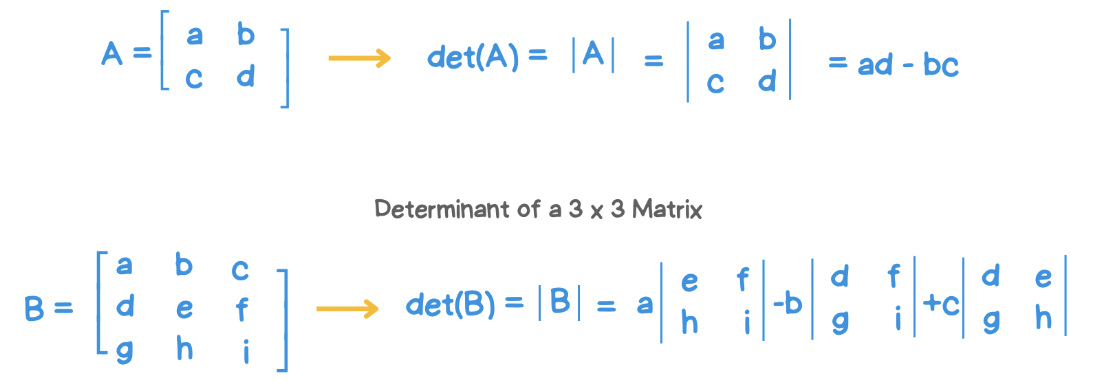
\includegraphics[scale = 0.5]{det.png}}\\
\end{center}
\end{tcolorbox}
\begin{tcolorbox}[colback=blue!5!white,colframe=blue!70!black,title= 8. Mátrix inverze]
    Az \(A \in M_{n\times n}\) mátrix inverzén \(A^{-1}\)-gyel jelölt \(n \times n\)-es mátrixot értünk, amelyre igaz, hogy:
    $$\underline{\underline{A}} * \underline{\underline{A}}^{-1} = \underline{\underline{A}}^{-1} * \underline{\underline{A}} = \underline{\underline{E}}$$
    \begin{center}
        \fbox{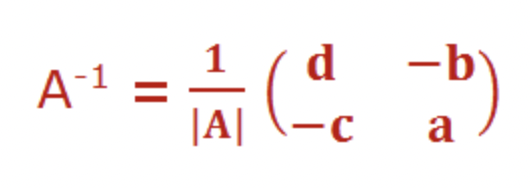
\includegraphics[scale = 0.7]{inverse.png}}\\
    \end{center}
\end{tcolorbox}

\begin{tcolorbox}[colback=blue!5!white,colframe=blue!70!black,title= 9. Mátrix rangja]
    A mátrix rangjának nevezzük a mátrix vektorai közül lineárisan függetlenek maximális számát.
    \begin{center}
        \fbox{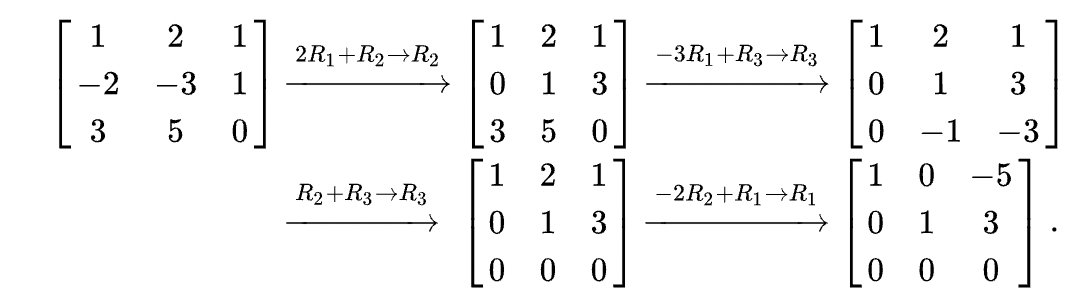
\includegraphics[scale = 0.5]{rank.png}}\\
        Az alábbi mátrix rangja 2.
    \end{center}
\end{tcolorbox}
\newpage

\textbf{Lineáris algebra II:}
\begin{tcolorbox}[colback=blue!5!white,colframe=blue!70!black,title= 1. Lineáris leképezés fogalma]
    \(V_1\) és \(V_2\) ugyanazon test \((\mathbb{R};\mathbb{C})\) feletti vektortérnek. Legyen \(V_1\to V_2\) leképezés, melyet lineáris leképezésnek nevezzük, ha:
    $$\varphi(\underline{a}+\underline{b}) = \varphi (\underline{a}) + \varphi(\underline{b})$$
    $$\varphi (\alpha \underline{a}) = \alpha \varphi(\underline{a})$$
    Megjegyzés: $$\varphi(\underline{0}) = \underline{0}$$
\end{tcolorbox}
\begin{tcolorbox}[colback=blue!5!white,colframe=blue!70!black,title= 2. Rang-nullitás tétele]
    Tetszőleges \(\varphi : V_1 \to V_2\) leképezés esetén igaz, hogy: \(def(\varphi)+rg(\varphi) = dim(V_1)\). Ebből \(def(\varphi)\) a magtér rangja. A magtér
\(V_1\) részhalmaza, és a benne lévő elemek képe nullvektor. A képtér \(V_2\) részhalmaza, és a benne lévő elemek a képei \(V_1\) elemeinek.
\end{tcolorbox}
\begin{tcolorbox}[colback=blue!5!white,colframe=blue!70!black,title= 3. Magtér]
    \textbf{Magtér:} Legyen \(\varphi : V_1 \to V_2\) lineáris leképezés:
    $$Ker(\varphi) := \{\underline{v}\mid \underline{v} \in V_1 \wedge \varphi(\underline{v}=\underline{0})\} $$
    a \(\varphi\) magtere.
\end{tcolorbox}
\begin{tcolorbox}[colback=blue!5!white,colframe=blue!70!black,title= 4. Sajátvektor{,} sajátérték]
    \begin{enumerate}
        \item A mátrixnak \(\lambda\) a sajátértéke, ha létezik olyan \(\underline{v}\) nem nulla vektor, hogy: \(\underline{\underline{A}} * \underline{v} = \lambda *\underline{v}\)
        \item Képlet:
        $$A' = \underline{\underline{C}}^{-1} * \underline{\underline{A}} * \underline{\underline{C}}$$
        \item \(\varphi: V \to V\) keressünk azon vektorokat, amelyekre igaz: \((A-\lambda \underline{\underline{E}})*\underline{v} = 0\). Ennek akkor van megoldása, ha:
        $$det(\underline{\underline{A}}-\lambda\underline{\underline{E}})=0$$
        \item Egy vektornak \(\infty\) saját vektora van. Lineárisan független egyenletrendszerek száma: \(\underline{\underline{A}}_{m\times n}\to max\) n db
        \item \(\alpha\)-t a \(v\) sajátvektorhoz tartozó sajátértéknek mondjuk.
    \end{enumerate}
\end{tcolorbox}
\begin{tcolorbox}[colback=blue!5!white,colframe=blue!70!black,title= 5. Bázistranszformáció]
    Legyen \( \{ \underline{b}_1, ..., \underline{b}_n \}\) és \(\{\hat{ \underline{b}}_1, ..., \hat{\underline{b}}_n \}\)bázis \(V\)-ben, ekkor az egyikről a másikra való áttérés \(S\) mátrixa:
    $$\hat{\underline{b}}_1 = \sum_{i = 1}^{n} s_i \underline{b}_i  $$
    $$\hat{\underline{b}}_1 = \sum_{i = 1}^{n} s_{ij} \underline{b}_i  $$
    $$\hat{\underline{b}}_1 = \sum_{i = 1}^{n} s_{in} \underline{b}_i  $$
    $$\begin{pmatrix}
        s_{1,1} & s_{1,2}  &...  & s_{1,n} \\
        s_{2,1} &s_{2,2}  &...  & s_{2,n} \\ 
        \vdots & \vdots  &  \ddots &  \\
        s_{n,1}&s_{n,2}  & ... & s_{n,n}
        \end{pmatrix}$$
\end{tcolorbox}
\begin{tcolorbox}[colback=blue!5!white,colframe=blue!70!black,title= 6. Hasonló mátrix]
    \(A\) és \(B\) mátrixok hasonlóak, ha létezik olyan \(X\) reguláris mátrix, hogy:
    $$\underline{\underline{A}} = \underline{\underline{X}}^{-1}* \underline{\underline{B}}*\underline{\underline{X}}$$
\end{tcolorbox}
\begin{tcolorbox}[colback=blue!5!white,colframe=blue!70!black,title= 7. Ortogonális mátrix]
    Egy mátrix ortogonális, amennyiben inverze megegyezik a transzponáltjával.  
\end{tcolorbox}
\newpage
\textbf{Függvénysorozatok, függvénysorok:}
\begin{tcolorbox}[colback=blue!5!white,colframe=blue!70!black,title= 1. Függvénysorozat]
    Az \(f_n : I \subset \mathbb{R}\to \mathbb{R}\) sorozatot függvénysorozatnak nevezünk. 
\end{tcolorbox}
\begin{tcolorbox}[colback=blue!5!white,colframe=blue!70!black,title= 2. Függvénysor]
Az \(f_n : I \subset \mathbb{R} \to \mathbb{R}\) függvény sorozat előállítható a:
$$s_1(x) := f_1(x)$$
$$s_2 := f_1(x)+f_2(x)$$
$$s_n(x) := \sum_{i=1}^i f_n(x)$$
az így előállított \(s_n\) sorozatot az \(f_n\) sorozatból képzett függvény sornak hívjuk, és \(\sum F_n\)-nel jelöljük.
\end{tcolorbox}
\begin{tcolorbox}[colback=blue!5!white,colframe=blue!70!black,title= 3. Függvénysorozat{,} függvénysor konvergenciája{,} egyenletes konvergenciája]
    A \(\sum f_n\) függvény sor egyenletesen konvergens az \(E \subset H\) halmazon \(\Longleftrightarrow\)  ha bármely \(\varepsilon > 0\) esetén létezik
olyan \(N(\varepsilon) : \mid s_n(x) - s_m(x)\mid < \varepsilon\); ha \(n;m > N(\varepsilon)\); \(\forall x \in E\) esetén.
\end{tcolorbox}
\begin{tcolorbox}[colback=blue!5!white,colframe=blue!70!black,title= 4. Weierstrass-tétel]
    Bármely \(f_n : I \subset \mathbb{R} \) és \(\sum f_n\) a belőle képzett függvénysor,\(\sum a_n\) olyan konvergens numerikus sor, amelyre igaz: \(\mid f_n(x)\mid \leq
a_n\); \(\forall x \in J\) esetén teljesül bármely \(x \in \mathbb{N}\) vagy egy bizonyos \(n\)-től, ekkor
\(\sum f_n\) függvénysor egyenletesen konvergens \(J\)-n.
\end{tcolorbox}
\begin{tcolorbox}[colback=blue!5!white,colframe =blue!70!black,title= 5. Cauchy-Hadamard-tétel]
    Legyne \(r\) a \(\sum_n x^n\) hatványsor konvergenciasugara:
    \begin{enumerate}
        \item Ha \(r = 0\) ebben az esetben a hatványsor csak az \(x_0\) pontban konvergens
        \item Ha \(r = \infty \) a hatványsor bármyel \(x_0 \in \mathbb{R}\) esetén konvergens 
        \item Hat \(0< r < \infty\), akkor a hatványsor abszolúz konvergens, ha \(\mid x\mid < r\), és divergens, amennyiben \(\mid x\mid >r\)
        \item Bizonyítás: az \(a,b\) rész bizonyítása az előző tétel alapján könnyen adódik:
        \begin{center}
            \(! \mid x_0\mid < r, limsup \sqrt[n]{\mid a_n x_0^n\mid} = \mid x_0 \mid limsup\sqrt[n]{\mid a_n \mid} = \frac{\mid x_0 \mid}{r}\), ami \(\mid x \mid > r \Rightarrow \)
        \end{center}
        Létezik olya \(0 < r < 1\), hogy a \(\sum a_x x_0^n\) hatványsor a gyökteszt miatt konvergens. Mivel \(\mid x_0 \mid < r\) tetszőleges volt, így \(\forall \mid x_0 \mid < r\) esetén igaz, hogy \(\sum a_n x_0^n\) hatványsor konvergens, amennyiben \(\mid x \mid > r\), akkor a hatványsor divergens.
    \end{enumerate}
\end{tcolorbox}
\begin{tcolorbox}[colback=blue!5!white,colframe=blue!70!black,title= 6. Hatványsor]
Tegyük fel, hogy egy \(f\) függvény \(\sum a_n x^b\) hatványsor alakban előállítható. Akkor az ezt leíró hatványsor alakja az alábbi: 
$$f(x) = \sum_{n=0}^{\infty} \frac{f^n(0)}{n!} *x^n$$
\end{tcolorbox}
\begin{tcolorbox}[colback=blue!5!white,colframe=blue!70!black,title= 7. Taylor-polinom{,} Taylor-sor]
Legyen \(f: I \subset \mathbb{R} \to \mathbb{R}\) függvény, az \(x_0 \in I\) pontban legfeljebb \(p\)-szer differenciálható, ekkor  az \(f\) függvények \(x_0\) körüli \(p\)-edik Taylor polinomja:
$$T_{f,P}(x) = \sum_{k=0}^P \frac{f^(k)}{k!}* (x-x_0)^k$$
\textbf{Tétel:} ha az \(f\) függvény legalább \((r+1)\)-szer differenciálható az \((x, x_0)\) intervallumon, és \(f^(k), k \in 1, 2, 3, ... r\) folytonos és az \(x\) és \(x_0\) pontokban, akkor létezik olyan \(\xi \in (x; x_0)\), hogy:
$$f(x) = \sum_{k=1}^r \frac{f^{(k)}x_0}{k!}* (x-x_0)^k + \frac{f^{(r+1)}\xi}{(r+1)!}(x-x_0)^{r+1}$$
Ahol a masodik tag a Lagrange-féle maradéktag 
\end{tcolorbox}
\begin{tcolorbox}[colback=blue!5!white,colframe=blue!70!black,title= 8. Konvergencia sugár{,} konvergencia tartomány]
Konvergencia sugár nagyságának kiszámítása:
$$\frac{1}{r} = lim_{m \to \infty} \mid \frac{a_{k +1}}{a_k} \mid$$
\end{tcolorbox}
\begin{tcolorbox}[colback=blue!5!white,colframe=blue!70!black,title= 9. Fourier-sor]
Legyen \( f : \mathbb{R} \to \mathbb{R}\) \(2l\) szerint periodikus függvény, amely a \([0, 2l]\) intervallumon Reimann integrálható, ekkor \(f\) Fourier során az alábbi függvénysort értjük:
$$ a_0 + \sum_{k=0}^{\infty} a_k\cdot cos(\frac{k\pi x}{l}) + b_k\cdot sin(\frac{k \pi x}{l})$$
$$a_0 = \frac{1}{2l} \int_{0}^{2l} f(x)\,dx; \hspace{10pt}b_0 = 0 $$
$$a_k = \frac{1}{l} \int_{0}^{2l} f(x)* cos(\frac{k \pi x}{l})\,dx;$$
$$b_k = \frac{1}{l} \int_{0}^{2l} f(x)* sin(\frac{k \pi x}{l})\,dx;$$
\textbf{Megjegyzés:} ha az \(f\) függvény összeáll a fenti típusú függvénysor összegeként, akkor az együtthatók csak ilyenek lehetnek.
\begin{center}
    \fbox{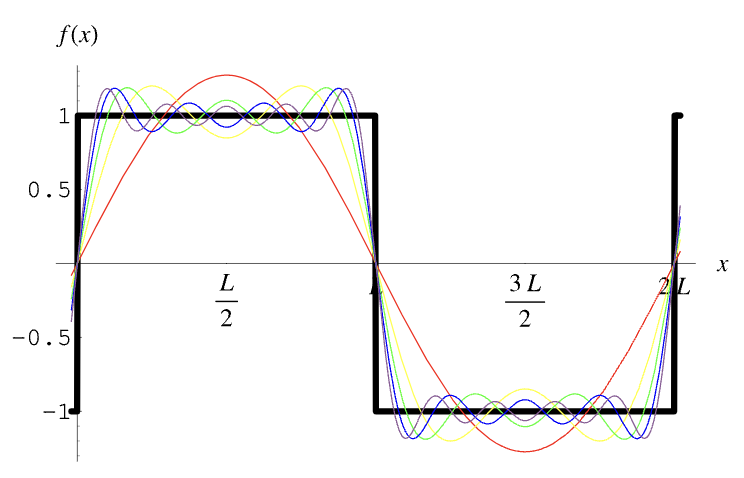
\includegraphics[scale = 0.7]{fourier.png}}
\end{center}
\end{tcolorbox}

\newpage
\textbf{Többváltozós függvények:}

\begin{tcolorbox}[colback=blue!5!white,colframe=blue!70!black,title= 1. Primitív függvény]
Egy \(f : \mathbb{R}^n \to \mathbb{R}^k\) függvénynek \(F: \mathbb{R}^n \to \mathbb{R}\) primitív függvénye, ha \(F'= f\).
\end{tcolorbox}
\begin{tcolorbox}[colback=blue!5!white,colframe=blue!70!black,title= 2. \(\mathbb{R}^n \to \mathbb{R}^k \) leképezés differenciálhatósága]
    Legyen \(U \subset \mathbb{R}^n\) nyílt halmaz, \(f : U \to \mathbb{R}^k\) leképezés. Azt mondjuk, hogy \(f\) differenciálható, az \(\underline{a} \in D_f\) pontban,
    ha létezik \(A: \mathbb{R}^n \to \mathbb{R}^k\) lineáris leképezés, \(\omega : \mathbb{R}^n \to \mathbb{R}^k\) leképezés, melyre \(\omega(\underline{0}) = \underline{0}\), \(Lim_{\mid\mid \underline{h}\mid \mid \to 0} \dfrac{\mid \mid \omega(\underline{h})\mid\mid}{\mid \mid \underline{h} \mid \mid}\),
    hogy:\\
    \begin{center}
        \(f(\underline{x}) - f(\underline{a}) = A(\underline{x} - \underline{a}) + \omega(\underline{x}- \underline{a})\). 
    \end{center}
    Az \("A"\)-nak megfelel egy \(M_{k\times n}\)-es mátrix. A deriválás egy leképezés.
\end{tcolorbox}
\begin{tcolorbox}[colback=blue!5!white,colframe=blue!70!black,title= 3. Iránymenti derivált]
    Az iránymenti derivált, az adott irány által kimetszett függvény deriváltja. Közelebbről:
    \begin{center}
        \(\dfrac{\partial f}{\partial \underline{e}} = Lim_{\lambda \to 0} \frac{f(\underline{x})+ \lambda \underline{e} - f(\underline{x})}{\lambda} = <\underline{e}, gradf>\), ahol \(\mid e\mid = 1\)
    \end{center}
    \begin{center}
        \fbox{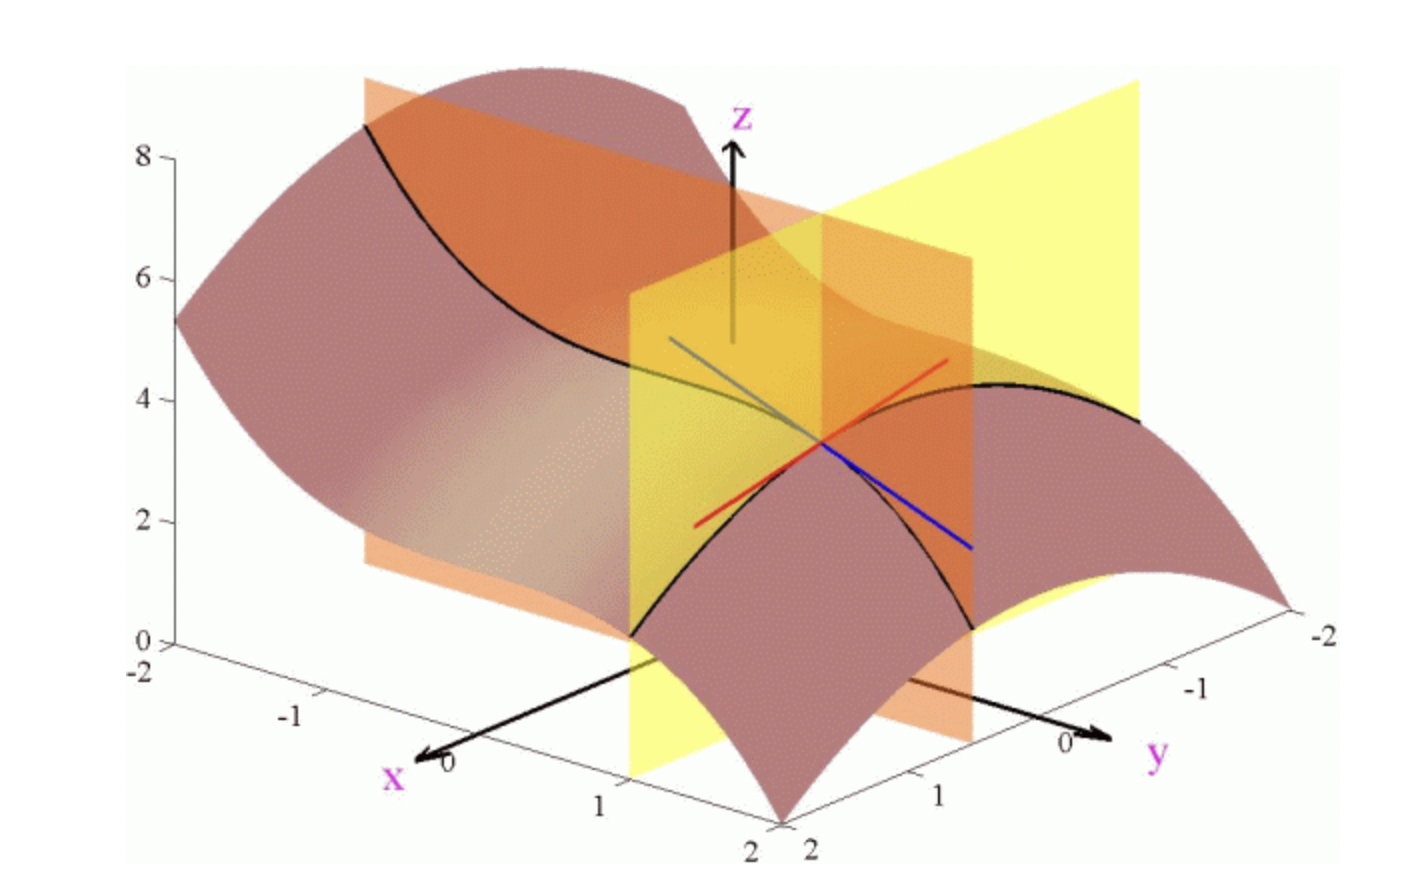
\includegraphics[scale = 0.3]{iranymenti.png}}\\
    \end{center}
\end{tcolorbox}
\begin{tcolorbox}[colback=blue!5!white,colframe=blue!70!black,title= 4. Parciális derivált]
    Parciális deriváltnak nevezzük a többváltozós függvények olyan deriváltját, amikor a függvényt egy rögzített változ
    ójának függvényeként fogjuk fel, eszerint deriválunk, miközben a többi változójelet konstans értéknek tekintjük. (A
    koordináta-tengelyek mentén lévő irány menti derivált.)
$$\frac{\partial f}{\partial x_i} = f'(x_i)$$
\end{tcolorbox}
\begin{tcolorbox}[colback=blue!5!white,colframe=blue!70!black,title= 5. Gradiens]
    A \(z = f(x; y)\) függvény gradiense a parciális deriváltakból, mint koordinátákból alkotott vektor: \(gradf(x; y) =
    (f'_x(x; y); f_y(x; y))\). A gradiens legfontosabb tulajdonságai:
    \begin{itemize}
        \item Minden pontban a gradiens merőleges a ponton áthaladó szimmetriavonalra.
        \item A gradiens a függvény legnagyobb növekedésének irányába mutat.
    \end{itemize}
    $$gradf = \bigtriangledown f = [f'x_1, ..., f'x_n]$$
\end{tcolorbox}
\begin{tcolorbox}[colback=blue!5!white,colframe=blue!70!black,title= 6. Jacobi-mátrix]
    A parciális deriváltak vektora vektor értékű függvényekre is defniálható. Ha \( \underline{F} : \mathbb{R}^n \to \mathbb{R}^m\) vektor értékű függvény,
    és koordinátafüggvényei rendre \(F_1; ...; F_m\), akkor:
    $$\underline{F}(x_1,...x_n) = (F_1(x_1,..., x_n), ... F_m(x_1, ..., x_n))$$
    Ekkor \(F\) deriváltja az \(F_i\) (sorvektor) gradiensek oszlopvektoraként definiálható. Ennek a mezőnek a vektorgradiense
a Jacobi -mátrix:
$$\mathcal{J}_{\underline{F}} = grad\underline{F} = \bigtriangledown \underline{F} = \partial (F_1, ..., F_m)\partial(x_1, ..., x_n) = \begin{pmatrix}
    \frac{\partial F_1}{\partial x_1} & ... &\frac{\partial F_1}{\partial x_n} \\ 
     \vdots & \ddots  &\vdots \\ 
    \frac{\partial F_m}{\partial x_1}& ... & \frac{\partial F_m}{\partial x_n}
    \end{pmatrix} $$
    \(m=n\)-re az eredmény egy másodfokú tenzor. Eféle tenzorok írják le például a fizikában a mechanikai feszültséget és
az elaszticitást.
\end{tcolorbox}
\begin{tcolorbox}[colback=blue!5!white,colframe=blue!70!black,title= 7. Szélsőérték{,} feltételes szélsőérték]
    A lokális szélsőérték létezésének szükséges feltétele, hogy az első rendű parciális deriváltak eltűnjenek az adott
    pontban. Emellett a létezés elégséges feltétel, hogy az adott a pontban a következő determináns értéke pozitív.
    $$H = \begin{vmatrix}
        f_{xx} & f_{xy} \\ 
        f_{yx} & f_{yy}
        \end{vmatrix}$$
        Egy \(f : \mathbb{R}^n \to \mathbb{R}\) függvénynek lokális minimuma van \(a\)-ban, ha \(a\)-nak van olyan \(K\) környezete, melyre \(f(a) \leq f(x)\forall x \in K\).\\\\
        Ha egy \(f \in c^1(\mathbb{R}^n;\mathbb{R})\) függvénynek lokális szélső értéke van \(a\)-ban, akkor \(f'(a) = 0\) a nullvektor, azaz \(\partial_i f(a) = 0(\forall i =
        1;\dots ; n)\)\\\\
        Legyen egy \(f \in C^2(\mathbb{R}^n;\mathbb{R})\) függvényre \(f'(a) = 0\)\\
        \begin{itemize}
            \item Ha \(F''(a)\) sajátértékei \(>0 \Rightarrow f\)-nek lokális minimuma van \(a\)-ban
            \item Ha \(F''(a)\) sajátértékei \(<0 \Rightarrow f\)-nek lokális maxima van \(a\)-ban
        \end{itemize}
        \textbf{Megjegyzés:} Többdimenziós jelenség ha \(f''(a)\)-nak van \(+\) és \(-\) sajátértéke is, akkor nincs szélsőértéke, hanem ún. nyeregpontja:
egy irányban minimum és egy másik irányban maximum van.

\begin{center}
    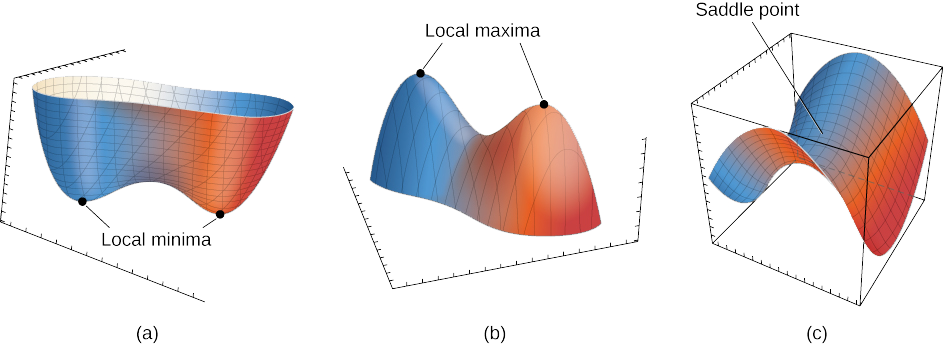
\includegraphics[scale = 0.8]{saddle_point.png}\\
\end{center}
\end{tcolorbox}
\begin{tcolorbox}[colback=blue!5!white,colframe=blue!70!black,title= 8. Kvadratikus formák definitsége]
Egy \(n\) változós \(q\) kvadratikus alakot:
\begin{enumerate}
    \item \textbf{pozitív definitnek} nevezünk, ha bármely \(x_1; \hdots ; x_n\) esetén \(q(x_1; \hdots ; x_n) \geq 0\), és \(q(x_1; \hdots ; x_n) = 0\) csak akkor,
    ha \(x_1 = \hdots = x_n = 0\)
    \item \textbf{pozitív szemidefinitnek} nevezzük, ha bármely \(x_1; \hdots ; x_n\) esetén \(q(x_1; \hdots ; x_n) \geq 0\), és van olyan \((x_1; \hdots ; x_n) \neq 0\),
    melyre igaz hogy: \(q(x_1; \hdots ; x_n) = 0\)
    \item \textbf{negatív definitnek} nevezzük, ha bármely \(x1; \hdots ; xn\) esetén \(q(x_1; \hdots ; x_n) \leq 0\), és \(q(x_1;\hdots ; x_n) = 0\), csak akkor
    ha: \(x_1 = \hdots = x_n = 0\)
    \item \textbf{negatív szemidefinitnek} nevezünk, ha bármely \(x_1;\hdots ; x_n\) esetén \(q(x_1; \hdots ; x_n) \leq 0\) és van olyan \((x_1; \hdots ; x_n) \neq 0\)
    melyre \(q(x_1; \hdots ; x_n) = 0\)
    \item \textbf{indefinitnek} nevezünk, ha felvesz pozitív és negatív értékeket is.
\end{enumerate}
\end{tcolorbox}
\begin{tcolorbox}[colback=blue!5!white,colframe=blue!70!black,title= 9. Riemann-integrálhatóság (alsó-felső Darboux-integrál)]
\begin{enumerate}
    \item \(\underline{S}(f) = inf\{\underline{S}(f,d)\mid d\) beosztása \(I\)-nek\(\}\)
    \item \(\underline{S}\) neve: alsó Darboux-integrál
    \item \(\overline{S}(f) = sup\{\overline{S}(f,d)\mid d\) beosztása \(I\)-nek\(\}\)
    \item \(\overline{S}\) neve: felső Darboux-integrál
\end{enumerate}
\textbf{Megjegyzés:}
$$\underline{S}(f,d) \leq \underline{S}(f) \leq \overline{S}(f) \leq \overline{S}(f,d) \forall d $$

Legyen \(f : \mathbb{R}^n \to \mathbb{R}\) korlátos függvény. \(f\)-et Riemann-integrálhatónak mondjuk, ha \(\underline{S}f = \overline{S}f\). Ezt a közös értéket
jelöljük.\\
\begin{center}
    \fbox{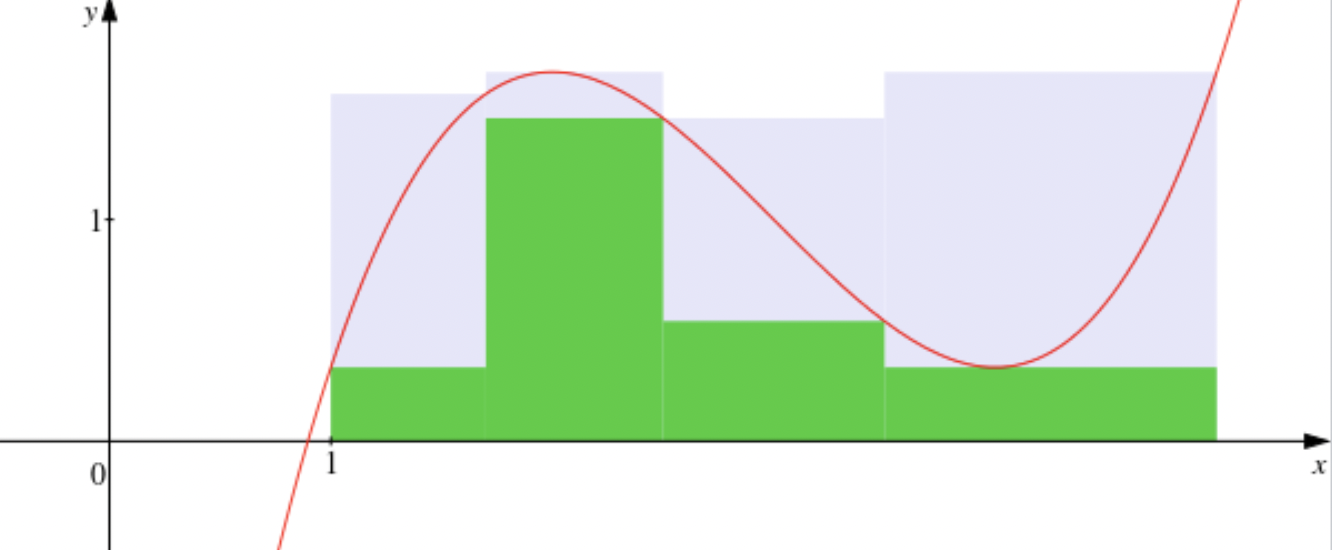
\includegraphics[scale = 0.5]{g2_4_9.png}}\\
    Alsó (zöld) és felső (zöld plusz levendula) Darboux összegek négy részintervallumra
\end{center}
\end{tcolorbox}

\newpage
\begin{center}
    \Large \textbf{Matematika G3 szóbeli beugró kérdések - 2023}
 \end{center}
 \setstretch{0.75}
 \textbf{Vektoranalízis 1.}
 \begin{enumerate}
    \item Duális tér
    \item Leképezés adjungáltja, szimmetrikus és antiszimmetrikus leképezés
    \item Mátrix vektorinvariánsa és nyoma (trace, spur)
    \item Gradiens, divergencia és rotáció
    \item Nabla vektor
    \item Laplace operátor, harmonikus függvény
 \end{enumerate}
 \textbf{Vektoranalízis 2.}
 \begin{enumerate}
    \item Skalárpotenciálos vektormező
    \item Vektorpotenciálos vektormező
    \item Görbe
    \item Görbe ívhossza
    \item Felület
    \item Felszínszámítás
    \item Stokes-tétel
    \item Gauss-Osztrogradszkij-tétel
    \item Green-tételek
 \end{enumerate}
 \textbf{Differenciálegyenletek 1.}
 \begin{enumerate}
    \item Közönséges n-edrendű differenciálegyenlet
    \item Differenciálegyenlet megoldásának típusai (általános, partikuláris, szinguláris)
    \item Cauchy-feladat
    \item Lipschitz-feltétel
    \item Picard-Lindelöf tétel
    \item Iránymező
 \end{enumerate}
 \textbf{Differenciálegyenletek 2.}
 \begin{enumerate}
    \item Szeparábilis és arra visszavezethető DE
    \item Bernoulli-féle DE
    \item Riccati-féle DE
    \item Egzakt DE
    \item Lineáris állandó együtthatós DE
    \item Lineárisan független függvényrendszer
    \item Wronski-determináns
    \item Differenciálegyenlet-rendszer
 \end{enumerate}

\newpage
\textbf{Vektoranalízis I:}

    \begin{tcolorbox}[colback=red!5!white,colframe=red!60!black,title= 1. Duális tér]
    $\mathbf{V}^* :=$ \textit{Hom}$(V,\mathbb{R})$, ahol $(V,+, \lambda)$ vektortér, $\mathbf{V}^*$ elemei pedig lineáris formák, azaz:
    $$\underline{v} \rightarrow \varphi(\underline{v})$$
    $$\varphi(\alpha\underline{v} + \beta\underline{w}) = \alpha\varphi(\underline{v}) + \beta\varphi(\underline{w})$$
    \begin{itemize}
        \item \textbf{Homomorfizmus:} Két algebrai struktúra közötti művelettartó leképezés. \\
        Pl. ha az egyik struktúrában valamely elemek közt valamilyen reláció áll fenn, akkor ezen elemeiknek képei a másik struktúrában is ebben a relációban állnak.
        \item \textbf{Endomorfizmus:} A képhalmaz részhalmaza az alaphalmaznak. pl: $\mathbb{Z} \rightarrow \mathbb{N}$
    \end{itemize}
    $V^*$ halmazt természetes módon vektortérré tehetjük a következőképpen:
    $$(\alpha + \beta )\underline{v} = \alpha\underline{v} + \beta\underline{v} \quad\quad \alpha,\beta \in \mathbf{V}^*$$
    $$(\rho \cdot \varphi)\underline{v} = \rho \cdot \varphi(\underline{v}) \quad\quad \rho \in \mathbb{R}, \varphi \in \mathbf{V}^*$$
    Így $(\mathbf{V}^*, +, \lambda)$ már vektortér, amit $V$ duális terének is nevezünk. Vektortér és duális terének dimenziója megegyezik. 
    \end{tcolorbox}

    \begin{tcolorbox}[colback=red!5!white,colframe=red!60!black,title= 2. Leképezés adjungáltja{,} szimmetrikus és antiszimmetrikus leképezés]
    \textbf{Leképezés adjungáltja:} \\
        Legyen $E = (V, <,>)$ adott euklédeszi tér és $\varphi:V \rightarrow V$ egy lineáris leképezés. \\
        Ekkor $\varphi^*:V \rightarrow V$ a leképezés adjungáltja ha $\forall \ \underline{v_1}, \underline{v_2} \in V$ esetén: \\
        $$<\underline{v_1}; \varphi(\underline{v_2})> = <\varphi^*(\underline{v_1}); \underline{v_2}>$$
        \begin{itemize}
            \item \textbf{Idempotens:} Az adjungált adjungáltja megegyezik az eredeti leképezéssel. $(\varphi^*)^* = \varphi$
        \end{itemize}
    \textbf{Szimmetrikus leképezés:} \\
        Egy leképezés szimmetrikus, ha adjungáltja önmaga $\varphi^* = \varphi$ ekkor:
        $$<\underline{v_1}; \varphi(\underline{v_2})> = <\varphi(\underline{v_1}); \underline{v_2}> \quad\quad \forall \ \underline{v_1}, \underline{v_2} \in V$$
    \textbf{Antiszimmetrikus leképezés:} \\
        Egy leképezés antiszimmetrikus, ha $\varphi^* = -\varphi$ ekkor:
        $$-<\underline{v_1}; \varphi(\underline{v_2})> = <\varphi(\underline{v_1}); \underline{v_2}> \quad\quad \forall \ \underline{v_1}, \underline{v_2} \in V$$ 
    \end{tcolorbox}

    \begin{tcolorbox}[colback=red!5!white,colframe=red!60!black,title= 3. Mátrix vektorinvariánsa és nyoma (trace{,} spur)]
    \textbf{Vektorinvariáns:} \\
    Tekintsük a következő, 3x3-as antiszimmetrikus mátrixnak és a $\underline{w}$ vektornak a szorzatát:
    $$\begin{bmatrix}
        0 & a_{12} & a_{13}\\
        -a_{12} & 0 & a_{23}\\
        -a_{13} & -a_{23} & 0
    \end{bmatrix} \cdot 
    \begin{bmatrix}
        w_1\\
        w_2\\
        w_3
    \end{bmatrix} = 
    \begin{bmatrix}
        a_{12}w_2 + a_{13}w_3\\
        -a_{12}w_1 + a_{23}w_3\\
        -a_{13}w_1 - a_{23}w_2
    \end{bmatrix}$$
    Egy antiszimmetrikus lineáris transzformáció mindig leírható egy rögzített vektorral való vektoriális szorzatként. Ezt a vektort nevezzük a mátrix vektorinvariánsának.
    $$\begin{bmatrix}
        v_1\\
        v_2\\
        v_3
    \end{bmatrix} \times
    \begin{bmatrix}
        w_1\\
        w_2\\
        w_3
    \end{bmatrix} =
    \begin{bmatrix}
        v_2w_3 - v_3w_2\\
        v_3w_1 - v_1w_3\\
        v_1w_2 - v_2w_1
    \end{bmatrix} $$
    $$\underline{\underline{A}} \cdot \underline{w} = \underline{v} \times \underline{w}$$
    $\underline{w}$ együtthatóinak meg kell egyeznie, tehát a vektorinvariáns: \\
    $$\underline{v}
    \begin{bmatrix}
        v_1\\
        v_2\\
        v_3
    \end{bmatrix} = 
    \begin{bmatrix}
        -a_{23}\\
        a_{13}\\
        -a_{12}
    \end{bmatrix}$$
    A vektorinvariáns csak ortogonális transzformációkkal szemben invariáns. \\\\
    \textbf{Nyom /Spur /Trace:} \\
    Egy lineáris transzformáció mátrixának főátlójában lévő elemek összege minden koordinátarendszerben ugyanannyi, tehát a koordináta-transzformációkkal szemben invariáns. \\
    Ezt az összeget a lineáris transzformáció $(V_{1}=V_{2})$ első skalárinvariánsának /nyomának /spurjának /tracejének nevezzük. (És ez a sajátértékek összege.)
    \begin{center}
        \fbox{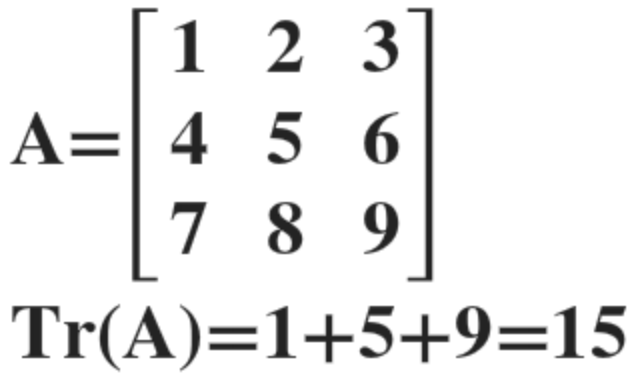
\includegraphics[scale= 0.5]{trace.png}}
    \end{center}
\end{tcolorbox}

    \begin{tcolorbox}[colback=red!5!white,colframe=red!60!black,title= 4. Gradiens{,} divergencia{,} rotáció I.]
    \textbf{Gradiens:} \\
    A gradiens csak skalármező (azaz skalár-vektor függvény) esetében értelmezhető.
    $$u:\mathbb{R}^3 \rightarrow \mathbb{R}$$
    $$grad\ u = \frac{\partial u}{\partial x}\textbf{i} + \frac{\partial u}{\partial y}\textbf{j} + \frac{\partial u}{\partial z}\textbf{k}$$
    A gradienst tehát úgy kapjuk, hogy a skalármezőt az összes változója szerint, külön-külön \\
    (parciálisan) lederiváljuk, és egy oszlopvektorba rendezzük.
    $$grad\ u =
    \begin{pmatrix}
        \dfrac{\partial u}{\partial x}\\[8pt]
        \dfrac{\partial u}{\partial y}\\[8pt]
        \dfrac{\partial u}{\partial z}
    \end{pmatrix}$$
    A gradiens tehát vektormennyiség. Ha bevezetjük az úgynevezett nabla vektort:
    $$\underline{\nabla} = 
    \begin{pmatrix}
        \dfrac{\partial}{\partial x}\\[8pt]
        \dfrac{\partial}{\partial y}\\[8pt]
        \dfrac{\partial}{\partial z}
    \end{pmatrix}$$
    Akkor $grad\ u$ a nabla vektornak és az $u$ skalármezőnek a szorzataként írható fel:
    $$grad\ u = \underline{\nabla} \cdot u$$
    Skalármező gradiense, illetve vektormező divergenciája és rotációja független a koordinátarendszertől.\\

    \textbf{Divergencia:} \\
    A divergencia csak vektormező (azaz vektor-vektor függvény) esetében értelmezhető. Eredménye skalármennyiség.
    $$\underline{v}: \mathbb{R}^3 \rightarrow \mathbb{R}^3 $$
    Definíció szerint $div\ \underline{v} = sp(\underline{\underline{\mathcal{J}_v}})$, tehát $\underline{v}$ Jakobi-mártixának a nyoma:
    $$div\ \underline{v} = \frac{\partial f_1}{\partial x} + \frac{\partial f_2}{\partial y} + \frac{\partial f_3}{\partial z}$$
    Ahol $f_i$ a $\underline{v}$ vektormező $i$-edik komponensfüggvénye. \\
    $div\ \underline{v}$ a nabla vektornak és a $\underline{v}$ vektormezőnek a (skaláris) szorzataként írható fel:
    $$div\ \underline{v} = \underline{\nabla} \cdot \underline{v}(\underline{r})$$
    Ha $div\ \underline{v} = 0$, akkor a vektormező forrásmentes.
\\\\
    \textbf{Rotáció:} \\
    A rotáció csak vektormező (azaz vektor-vektor függvény) esetében értelmezhető. Eredménye viszont vektormennyiség. \\
    Definíció szerint $\frac{1}{2}rot\ f = \frac{1}{2}(Df-Df^*)$, ahol $Df$ a derivált mátrix (Jakobi-mátrix), aminek a soraiban az egyes komponensfüggvények gradiensei vannak. $Df^*$ pegid $Df$ transzponáltja. \\
    $rot\ \underline{v}$ a nabla vektornak és a $\underline{v}$ vektormezőnek a vektoriális szorzataként írható fel:
    $$rot\ \underline{v} = \underline{\nabla} \times \underline{v}(\underline{r})$$
    \end{tcolorbox}

    \begin{tcolorbox}[colback=red!5!white,colframe=red!60!black,title= 4. Gradiens{,} divergencia{,} rotáció II.] %folyatása az előzőnek (nem tudja a latex törni a blokkokat)
    $\underline{v}: \mathbb{R}^3 \rightarrow \mathbb{R}^3$ esetén:
    $$rot\ \underline{v} = 
    \begin{pmatrix}
        \dfrac{\partial f_z}{\partial y} - \dfrac{\partial f_y}{\partial z}\\[8pt]
        \dfrac{\partial f_x}{\partial z} - \dfrac{\partial f_z}{\partial x}\\[8pt]
        \dfrac{\partial f_y}{\partial x} - \dfrac{\partial f_x}{\partial y}
    \end{pmatrix}$$
    Fontosabb azonosságok: $\underline{r} = \begin{pmatrix} x\\ y\\ z \end{pmatrix}$
    $$div\ \underline{r} = 3$$
    $$rot\ \underline{r} = 0$$
    Zérus azonosságok:
    $$rot\,grad\ u = \underline{0}$$
    $$div\,rot\ \underline{v} = 0$$
    \end{tcolorbox}

    \begin{tcolorbox}[colback=red!5!white,colframe=red!60!black,title= 5. Nabla vektor]
    Igazából nem vektor, hanem operátor, de vektorként kezelve a legtöbb művelet könnyebben
    elvégezhető a segítségével.
    $$\underline{\nabla} = 
    \begin{pmatrix}
        \dfrac{\partial}{\partial x}\\[8pt]
        \dfrac{\partial}{\partial y}\\[8pt]
        \dfrac{\partial}{\partial z}
    \end{pmatrix}$$
    \end{tcolorbox}

    \begin{tcolorbox}[colback=red!5!white,colframe=red!60!black,title= 6. Laplace operátor{,} harmonikus függvény]
    \textbf{Laplace operátor:}
    $$\Delta = \underline{\nabla} \cdot \underline{\nabla} = \frac{\partial^2}{\partial x^2} + \frac{\partial^2}{\partial y^2} + \frac{\partial^2}{\partial z^2}$$
    \textbf{Harmonikus függvény:} \\
    Akkor harmonikus például az $u$ skalár-vektor $(\mathbb{R}^3 \rightarrow \mathbb{R})$ függvény, ha:
    $$\Delta u = 0 = \underline{\nabla} \cdot \underline{\nabla}u = \underline{\nabla} \cdot grad\ u = div\,grad\ u = 0$$
    Tehát kielégíti az úgynevezett Laplace-egyenletet. (Feltétel: legyen kétszeresen differenciálható az $u$ függvény.)
    \end{tcolorbox}

\newpage
\textbf{Vektoranalízis II:}

    \begin{tcolorbox}[colback=red!5!white,colframe=red!60!black,title= 1. Skalárpotenciálos vektormező]
    Egy $\underline{v}:V \rightarrow V$ vektormező skalárpotenciálos, ha $\exists\ u: V \rightarrow \mathbb{R}$ skalármező, hogy $\underline{v} = grad\ u$.\\
    (Fizikai) erőtér esetén a vektortér más néven konzervatív, ha ez teljesül.\\
    Ekkor $u$-t $\underline{v}$ potenciálfüggvényének nevezzük. Feltétel: $rot\ \underline{v} = \underline{0}$ (örvénymenteség) \\
    Ha egy vektormező előáll egy skalármező gradienseként, akkor a vektormező bármely görbe menti skalárértékű vonalintegrálja csak a kezdő- és a végponttól függ, tehát független az úttól.\\
    Egy vektortérnek végtelen sok skalárpotenciálja van (a konstans miatt).\\ 
    A skalárértékű vonalintegrál értéke (a munka) a potenciálkülönbséggel egyenlő:
    $$\int_{A}^{B} <\underline{v}(\underline{r}(\underline{t})), \underline{\dot{r}}(t)> = u(B) - u(A)$$
    A potenciálfüggvénynek a vonalintegrállal kapcsolatban az a szerepe, mint egy egyváltozós függvény határozott integráljával kapcsolatban a primitív függvénynek.
    \end{tcolorbox}

    \begin{tcolorbox}[colback=red!5!white,colframe=red!60!black,title= 2. Vektorpotenciálos vektormező]
        Egy $\underline{v}:V \rightarrow V$ vektormező vektorpotenciálos, ha $\exists\ \underline{w}: V \rightarrow V$ vektormező, hogy $\underline{v} = rot\ \underline{w}$, azaz előáll egy másikmező rotációjaként. ($\underline{w}$ vektor tetszőleges koordinátáját nullának választjuk a megoldás során.)
        Feltétele: $div\ \underline{v} = 0$. (forrásmenteség)
    \end{tcolorbox}

    \begin{tcolorbox}[colback=red!5!white,colframe=red!60!black,title= 3. Görbe]
        Legyen $I \in \mathbb{R}$ egy nem feltétlenül korlátos intervallum. Ekkor az $\underline{r}:I \rightarrow \mathbb{R}^3$ leképezést reguláris görbének hívjuk, ha $r$ immerzió, azaz a derivált leképezése injektív (a képek egyenlőségéből következik az ősképek egyenlősége: $\varphi(a) = \varphi(b) \rightarrow a = b$).
    \end{tcolorbox}

    \begin{tcolorbox}[colback=red!5!white,colframe=red!60!black,title= 4. Görbe ívhossza]
        A pályasebesség $I$ fölötti integrálját a térgörbe ívhosszának nevezzük (sebesség idő szerinti vonalintegrálját):
        $$L(\underline{r}) = \int_{I}\left|\left|\dot{\underline{r}}(\tau)\right|\right|d\tau$$
        Más definíció szerint, amikor egy tetszőleges síkgörbe ívhosszát olyan húrok összegével közelítjük, amik 0-hoz tartanak.\\
        Egy $y = f(x)$ egyenlettel adott, szakaszonként sima görbe $a \leq x \leq b$ határok közötti ívhossza:
        $$s = \int_{x=a}^{b} \,ds = \int_{x=a}^{b} \sqrt{1+y'^2} \,dx$$
        A „töröttvonalak” hosszának az összege is az ívhossz, minden határon túli finomítás esetén:
        $$\sum_{i}\left|\left|\underline{r}(t_i) - \underline{r}(t_{i-1})\right|\right|$$
    \end{tcolorbox}

    \begin{tcolorbox}[colback=red!5!white,colframe=red!60!black,title= 5. Felület]
        Legyen $S \subset \mathbb{R}^3$, ekkor $S$-t reguláris (szabályos) felületnek mondjuk, ha $\forall\ p \in S$ ponthoz létezik $p$-nek olyan $V \subset \mathbb{R}^3$ környezete, hogy a $\varphi:U \subset \mathbb{R}^2 \rightarrow V \cap S$ leképezés:
            \begin{itemize}
                \item differenciálható homeomorfizmus (diffeomorfizmus, azaz differenciálható bijekció)
                \item és $\varphi$ immerzió, azaz a $\varphi'_q:\mathbb{R}^2 \rightarrow \mathbb{R}^3$ ($q$ pontban) injektív lineáris leképezés\\
                $\varphi$ neve: parametrizáció, $p \in V \cap S$ neve: $p$ koordinátakörnyezete
            \end{itemize}
    \end{tcolorbox}

    \begin{tcolorbox}[colback=red!5!white,colframe=red!60!black,title= 6. Felszínszámítás]
        Triangularizáció (felszín lefedése háromszögekkel) helyett kicsi, elemi, érintő paralelogrammákkal közelítjük a felszínt, amik már nem tudnak elválni a felülettől (ez az alapelve). \\
        \textbf{Skaláris felületelem:}
        $$dS = \left|\left|\frac{\partial\underline{r}}{\partial u} \times \frac{\partial\underline{r}}{\partial v}\right|\right|\Delta u \Delta v$$
        Ahol $\frac{\partial\underline{r}}{\partial u}$ és $\frac{\partial\underline{r}}{\partial v}$ a paramétervonalak $P$ pontbeli érintővektorai. (A felületen a $P$ pontot az $u$ és $v$
        úgynevezett paramétervonalak metszéseként vettük fel; $\underline{r}$ a $P$ pontba mutató vektor). A skaláris felületelem a két differenciálvektor által kifeszített elemi paralelogramma területe. Amit, ha minden határon túl finomítunk, akkor a következő integrál megadja a teljes felszínt:
        $$S = \iint_{T}  \,dS = \iint_{T} \left|\left|\frac{\partial\underline{r}}{\partial u} \times \frac{\partial\underline{r}}{\partial v}\right|\right|dudv$$
    \end{tcolorbox}

    \begin{tcolorbox}[colback=red!5!white,colframe=red!60!black,title= 7. Stokes-tétel]
        A görbe menti és a felületi integrálok közötti kapcsolatot írja le. „Kétdimenziós Newton-Leibnizformulának” is szokták nevezni. \\
        Legyen $F: [a,b] \times [a,b] \rightarrow \mathbb{R}^3$ jobbkéz-szabály szerint irányított, parametrizált peremes felület Továbbá, legyen $\underline{v}: \mathbb{R}^3 \rightarrow \mathbb{R}^3$ legalább egyszer folytonosan differenciálható vektormező, ekkor:
        $$\oint_{\mathcal{G}}<\underline{v}(\underline{r}),d\underline{s}> \iint_{F}<rot\ \underline{v},d\underline{F}>$$
        Tehát a $\mathcal{G}$ görbe menti vonalintegrál megegyezik az $F$ felületen vett felületi integrállal. $d\underline{F} = \underline{n}$ Ezáltal is belátható, hogy ha a vektormező örvénymentes, akkor bármely zárt görbe menti integrálja zérus, hiszen, ha $rot\ \underline{v} = 0$, akkor a skalárszorzat nulla a kettős integrálban. \\
        \textbf{Megjegyzések:}
        \begin{itemize}
            \item Kétoldalú, zárt felület legyen adott, amit egy zárt görbe határol
            \item Azonos peremmel rendelkező $S_1$ és $S_2$ felületek esetén az integrálok megegyeznek
            \item Perem nélküli felület esetén nulla a kettős integrál értéke
            \item Ha nem irányítható a felület, akkor felbontjuk irányítható részekre
            \item Fizikai alkalmazás pl. gerjesztési törvény
        \end{itemize}
    \end{tcolorbox}

    \begin{tcolorbox}[colback=red!5!white,colframe=red!60!black,title= 8. Gauss-Osztrogradszkij-tétel]
        A felületi integrál és a térfogati integrál között teremt kapcsolatot. Szükséges egy korlátos, zárt felület és egy kifelé mutató normálvektor. Legyen $V: [a,b]^3 \rightarrow \mathbb{R}^3$ irányított, paraméterezett elemi tértartomány és $\underline{v}: \mathbb{R}^3 \rightarrow \mathbb{R}^3$ $V$-n legalább egyszer differenciálható vektormező, ekkor:
        $$\oiint_F <\underline{v}(\underline{r}),d\underline{F}> = \iiint_V div(\underline{v}(\underline{r}))dV$$
        Ahol $F$ a határfelülete $V$-nek. A tételből látható, hogy forrásmentes $(div\ \underline{v} = 0)$ vektortér zárt felületre vett integrálja (avagy átáramlási feleslege) nulla.
    \end{tcolorbox}

    \begin{tcolorbox}[colback=red!5!white,colframe=red!60!black,title= 9. Green-tételek]
        Legyenek $\varphi, \psi: \mathbb{R}^3 \rightarrow \mathbb{R}$ kétszeresen folytonosan differenciálható skalármezők. A Gauss-Osztrogradszkij-tételben vegyük fel a $\underline{v}$ vektorteret $\underline{v} = \varphi \cdot grad\ \psi$ alakban.
        $$div\ \underline{v} = \underline{\nabla} \cdot \underline{v} = \underline{\nabla}(\varphi \cdot \underline{\nabla}\psi) = \underline{\nabla}\varphi\underline{\nabla}\psi + \varphi\Delta\psi = grad\ \varphi grad\ \psi + \varphi\Delta\psi$$
        \textbf{Aszimmetrikus Green-tételt:}
        $$\oiint_{F} <\varphi \cdot grad\ \psi, d\underline{F}> = \iiint_{V}(grad\ \varphi\ grad\ \psi + \varphi\Delta\psi)dV$$
        Az első Green-tételben $\varphi$ és $\psi$ szerepét felcseréljuk, és az így kapott egyenletet kivonjuk az első tétel egyenletéből. \\
        \textbf{Szimmetrikus Green-tétel:}
        $$\oiint_{F} <\varphi \cdot grad\ \psi - \psi \cdot grad\ \varphi, d\underline{F}> = \iiint_{V}(\varphi\Delta\psi - \psi\Delta\varphi)dV$$
    \end{tcolorbox}

\newpage
\textbf{Differenciálegyenletek I:}

    \begin{tcolorbox}[colback=red!5!white,colframe=red!60!black,title= 1. Közönséges n-edrendű differenciálegyenlet]
        Differenciálegyenletnek az olyan egyenletet nevezzük, melyben ismeretlen függvények, ezek deriváltjai, valamint független változó(k) fordul(nak) elő. \\
        \textbf{Közönséges:} csak egyetlen független $(x)$ változó van benne (nem parciális, ahol több) \\
        \textbf{Rend:} az ismeretlen $(y', y'',\ \dots)$ legmagasabb fokszámú deriváltja \\
        \textbf{Definíció:} \\
        $y:\mathbb{R} \rightarrow \mathbb{R}$ $n$-szer folytonosan differenciálható függvény, $y = y^{(0)}, y' = y^{(1)}, \dots, y^{(n)}$ deriváltfüggvények szintén folytonosak és jelölje $x$ a független változót.
        $$F(x,y,y',y'',\dots,y^{(n)}) = 0$$
        egyenlet az $y$-ra vonatkozó, $n$-edrendű, közönséges differenciálegyenlet. (A fenti megadást implicit megadásnak is hívjuk, mivel a legmagasabb fokszámú derivált nem fejezhető ki egyértelműen, expliciten.)
    \end{tcolorbox}

    \begin{tcolorbox}[colback=red!5!white,colframe=red!60!black,title= 2. Differenciálegyenlet megoldásának típusai]
        \textbf{Általános:} \\
        Amely kielégíti a differenciálegyenletet (DE-t) és pontosan annyi, egymástól független, tetszőleges konstanst tartalmaz, ahányad rendű a DE. Az általános megoldás a homogén és az inhomogén rész összege: $y_{\acute{a} } = y_{H} + y_{IH}$ \\
        \textbf{Partikuláris:} \\
        Amely az általános megoldásból úgy származtatható, hogy az abban szereplő konstansoknak meghatározott értéket adunk. (pl. Cauchy kezdetiérték-feladat) Általánosabban: partikuláris megoldás, ha a megoldásfüggvény legalább 1-gyel kevesebb egymástól független állandót tartalmaz, mint ahányad rendű a DE. \\
        \textbf{Szinguláris:} \\
        Olyan megoldás, amely NEM kapható meg az általános megoldásból az állandók megfelelő választásával. (pl. szeparábilis DE esetén)
    \end{tcolorbox}

    \begin{tcolorbox}[colback=red!5!white,colframe=red!60!black,title= 3. Cauchy-feladat]
        Az $n$-edrendű DE olyan megoldását keressük, amely kielégíti:
        $$y(x_{0}) = y_{0}, y'(x_{0}) = y'_0,\dots, y^{(n-1)}(x_{0}) = y^{(n-1)}_0$$
        kezdeti feltételt, ahol $x_{0}, y_{0}, y'_{0},\dots, y^{(n-1)}_{0}$ adott számok. Egy DE megoldása során meg van adva megfelelő számú peremfeltétel (PF), amikkel az integrálás során feltűnő állandók értéke meghatározható. Annyi PF kell, ahányad rendű a DE.
    \end{tcolorbox}

    \begin{tcolorbox}[colback=red!5!white,colframe=red!60!black,title= 4. Lipschitz-feltétel]
        Ha az $f$ függvény teljesíti a Lipschitz-feltételt az adott tértartományon, akkor a megoldásgörbék nem metszik egymást (azaz létezik egyértelmű megoldás, egy ponton csak egy darab integrálgörbe halad át). \\
        \textbf{Definíció:} \\
        Az $f$ függvény a $D$ tartományon az $y$ változóra nézve kielégíti a Lipschitz-feltételt, ha létezik $M$ pozitív valós szám:
        $$\left|f(x,y_{2}) - f(x,y_{1})\right| \leq M\left|y_{2}-y_{1}\right| \quad\quad \forall\ (x,y_1),(x,y_2) \in D$$ 
    \end{tcolorbox}

    \begin{tcolorbox}[colback=red!5!white,colframe=red!60!black,title= 5. Picard-Lindelöf tétel]
        Ez egyben egzisztencia- és unicitástétel is. Legyen $y' = f(x,y)$ explicit alakban adott DE, és $D = I_1 \times I_2$ nyílt téglalap tartomány, ahol $I_1, I_2$ nyílt intervallumok és legyen $(x_0,y_0) \in D$, továbbá:
        \begin{itemize}
            \item $f$ folytonos mindkét változójában $D$-n.
            \item $f$ elégítse ki a Lipschitz-feltételt $y$ változóra $D$-n.
        \end{itemize}
        Egyértelműen létezik $\varphi: (x_0 - \varepsilon,x_0 + \varepsilon) \rightarrow \mathbb{R}$ függvény melyre,
        $$\varphi'(x) = f(x,\varphi(x))$$
        $$\varphi'(x_0) = y_0$$
        egyaránt teljesül, azaz a $\varphi$ megoldás egyértelmű. \\
        \textbf{Megjegyzések:}
        \begin{itemize}
            \item Ha $f$ függvényről csak a folytonosságot feltételezzük: Peano-feltétel.
            \item Hasonlóan a Cauchy-feltételhez (ott I. feltétel ugyanaz, II. feltétel, hogy az $f$ függvény $y$ szerinti parciális deriváltja korlátos $\forall\ D$-beli pontban), a Picard-Lindelöf tétel is erősebb, szigorúbb tétel. Hiszen, a tételben elegendő, de nem szükséges feltételek vannak, ezáltal lehet, hogy nem teljesül mindkét feltétel, mégis van egyértelmű megoldás!
        \end{itemize}
    \end{tcolorbox}

    \begin{tcolorbox}[colback=red!5!white,colframe=red!60!black,title= 6. Iránymező]
        Az iránymező a differenciálegyenlet megoldásairól ad szemléletes képet. Az $y' = f(x,y)$ DE megoldása geometriailag a következőképpen szemléltethető. Az $f$ függvény értelmezési tartományának minden egyes $(x,y)$ pontjához rendeljük hozzá a rajta átmenő, $y' = f(x,y)$ iránytangensű (meredekségű) egyenesnek (megoldásgörbének) a pontot tartalmazó kicsiny szakaszát. E szakaszok összessége alkotja a differenciálegyenlet iránymezőjét; a szakaszokból elég sokat ábrázolva kapjuk a DE megoldásának geometriai képét.\\
        Tehát sok-sok pontban berajzoljuk az érintők egy kicsiny darabját, ezek lesznek a képen is látható vonalelemek, amik összessége az iránymező.\\
        \textbf{Izoklina:} Az a görbe, amelynek pontjaihoz azonos irányú, vagyis párhuzamos vonalelemek tartoznak.
        \begin{center}
            \fbox{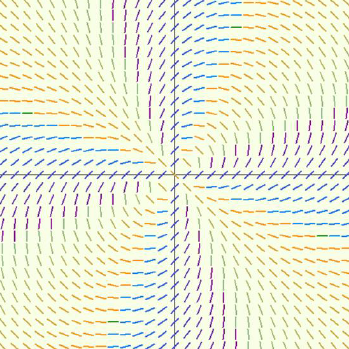
\includegraphics[scale = 0.6]{1_1_1.png}}
        \end{center}
    \end{tcolorbox}
\newpage
\textbf{Differenciálegyenletek II:}    

    \begin{tcolorbox}[colback=red!5!white,colframe=red!60!black,title= 1. Szeparábilis és arra visszavezethető DE]
        \textbf{Definíció:} \\
        Az olyan $y' = f(x,y)$ elsőrendű DE-et, amely $y' = h(x) \cdot g(y)$ alakra hozható, szeparábilis (változóiban szétválasztható) differenciálegyenletnek nevezzük. Feltesszük, hogy $h$ és $g$ valamely, alkalmas $I$ és $J$ intervallumon folytonosak. \\
        \textbf{Megoldás:} \\
        $$\dfrac{dy}{dx} = y' = h(x) \cdot g(y)$$
        $$\int\dfrac{1}{g(y)}dy = \int h(x)dx$$
        \textbf{Szinguláris megoldás:} $g(y) = 0$, amivel osztani kell \\
        \textbf{Nem szinguláris megoldás:} $g(y) \neq 0$ \\
        Szeparábilis differenciálegyenletre visszavezethetőek más DE-ek is $u$ helyettesítéssel:
        $$y' = f(ax + by + c)$$
        $$u := ax + by + c$$
        $$u' = \dfrac{du}{dx} = a + by' = a + b \cdot f(u)$$
        illetve
        $$y' = f(1,\dfrac{y}{x})$$
        $$u = \dfrac{y}{x}$$
        $$u' = \dfrac{du}{dx} = \dfrac{y'x - y \cdot 1}{x^2} = \dfrac{y'}{x} - \dfrac{y}{x^2} = \dfrac{y' - \dfrac{y}{x}}{x}$$
        Továbbá, fontos még az is, hogy az elsőrendű, lineáris differenciálegyenleteknek a homogén része is szétválasztható DE-re vezethető vissza.
    \end{tcolorbox}
    \begin{tcolorbox}[colback=red!5!white,colframe=red!60!black,title= 2. Bernoulli-féle DE]
       \textbf{Definíció:} \\
       Az $y' + p(x) \cdot y = q(x) \cdot y^n (n \neq 0, n \neq 1)$ alakú, elsőrendű, nemlineáris DE-et. Bernoulli-féle differenciálegyenletnek nevezzük, ahol $p, q: I \subset \mathbb{R} \rightarrow \mathbb{R}$ folytonos függvények. \\
       \textbf{Megoldás helyettesítéssel:} \\
       $$z(x) = z = y^{1-n} \quad\quad \text{(eredeti DE)}$$
       $$z' = \dfrac{dz}{dx} = (1-n) \cdot y^{-n} \cdot y' \quad\quad (1)$$
       Ahonnan az eredeti DE-et $y^n$-nel leosztva, a (1) egyenletet pedig $1-n$-nel leosztva és felhasználva a helyettesítést, azt kapjuk, hogy:
       $$z' + (1-n)p(x) \cdot z = (1-n)q(x)$$
       Ami már egy lineáris DE $z$-re nézve, tehát megoldható homogén-inhomogén módon.
    \end{tcolorbox}

    \begin{tcolorbox}[colback=red!5!white,colframe=red!60!black,title= 3. Riccati-féle DE]
        \textbf{Definíció:} \\
        Az $a(x) \cdot y' + b(x) \cdot y + c(x) \cdot y^2 = r(x)$ alakú elsőrendű, nemlineáris DE-et Riccatiféle
        differenciálegyenletnek nevezzük, ahol $a, b, c, r: I \subset \mathbb{R} \rightarrow \mathbb{R}$ folytonos függvények. \\
        \textbf{Megoldás:} \\
        A Riccati-féle nemlineáris DE integrálással általában nem oldható meg. Akkor, és csak akkor tudjuk integrálással előállítani a megoldását, ha ismerjük egy partikuláris megoldását. \\
        \textbf{Megjegyzések:}
        \begin{itemize}
            \item Ha $r(x) = 0$, akkor Bernoulli-féle DE-et kapunk
            \item Ha $c(x) = 0$, akkor a DE lineáris
        \end{itemize}
        $y(x) = \frac{1}{z(x)} + y_p(x)$ alakban bevezetett új függvény segítségével $z$-re már lineáris DE-et kapunk, vagy $y(x) =  z(x) + y_p(x)$ típusú helyettesítéssel Bernoulli-típusúra redukálható a Riccati-féle DE. \\
        \textbf{Megoldás helyettesítéssel:} \\
        $y' = x + z \rightarrow y' = 1 + z'$, amit visszaírva a DE-be, leegyszerűsödik Bernoulli-ra.
    \end{tcolorbox}

    \begin{tcolorbox}[colback=red!5!white,colframe=red!60!black,title= 4. Egzakt DE]
        \textbf{Definíció:} \\
        Egy $P(x, y)dx + Q(x, y)dy = 0$ lakú DE-et, melyben $P, Q: D \subset \mathbb{R}^2 \rightarrow \mathbb{R}$ folytonos függvények, egzakt DE-nek nevezzük, ha az alábbi két parciális derivált folytonos és egyenlőek:
        $$\dfrac{\partial P}{\partial y} = \dfrac{\partial Q}{\partial x}$$
        \textbf{Megoldás:} \\
        DE megoldása $F(x, y) = C$ alakú (a skalárpotenciál kereséséhez hasonló). Létezik olyan $F(x, y)$, hogy:
        $$\dfrac{\partial F}{\partial x} = P \quad \text{és} \quad \dfrac{\partial F}{\partial y} = Q$$
        \textbf{Egzaktra visszavezethető:} $P(x, y)dx + Q(x, y)dy = 0$ alakú DE általában nem egzakt (vagyis a bal oldala nem teljes differenciál), azaz:
        $$\dfrac{\partial P(x, y)}{\partial y} \neq \dfrac{\partial Q(x, y)}{\partial x}$$
        Ilyen esetben kísérletet tehetünk egy olyan $M(x, y) \neq 0$ függvény megkeresésére, amellyel a differenciálegyenletet beszorozva az új DE már egzakt lesz:
        $$ln\left|M(x)\right| = \int \dfrac{P'_y-Q'_x}{Q}dx$$
        $$ln\left|M(y)\right| = \int \dfrac{Q'_x-P'_y}{P}dy$$
        Azt a multiplikátort kell használni, ami csak az egyik változótól függ (amit ki lehet integrálni).
    \end{tcolorbox}

    \begin{tcolorbox}[colback=red!5!white,colframe=red!60!black,title= 5. Lineáris állandó együtthatós DE]
        \textbf{Lineáris:} az ismeretlen függvény és annak deriváltjai csak első hatványon szerepelnek és
        ezek szorzatai sem fordulnak elő az egyenletben. (Ellenkező esetben nemlineáris.) \\
        \textbf{Definíció:} \\
        Az $a_n \cdot y^{(n)} + a_{n-1} + \hdots + a_1 \cdot y' + a_0 \cdot y = 0$ DE-et, ahol $a_i \in \mathbb{R}, i \in \{0,1, \hdots n \}$ $n$-edrendű $(a_n \neq 0)$, állandó (konstans) együtthatós, lineáris differenciálegyenletnek hívjuk. \\
        Egy $n$-edrendű, állandó együtthatós lineáris differenciálegyenlet megoldásai $n$-dimenziós, valós vektorteret alkotnak a $\mathbb{R}$ fölött. Ezért elegendő $n$ darab lineárisan független megoldást megtalálni. Ezeket elemi megoldásoknak, más szóval alaprendszernek nevezzük.
    \end{tcolorbox}
    \begin{tcolorbox}[colback=red!5!white,colframe=red!60!black,title= 6. Lineárisan független függvényrendszer]
        Legyen \(y_1, y_2, \hdots, y_n:(a, b) \to \mathbb{R}; (a, b)\)-n \(n-1\)-szer folytonosan differenciálható függvénynrendszer. Ez az \(n\) db függvény lineárisan független ha:
        $$c_1y_1(x) + c_2y_2(x) + \hdots + c_ny_n(x) \equiv 0$$
        azonosság csakis a \(c_1 = c_2 = \hdots = c_n = 0\) esetben áll fenn. Ellenkező esetben a függvények lineárisan függők.
        
    \end{tcolorbox}
    \begin{tcolorbox}[colback=red!5!white,colframe=red!60!black,title= 7. Wronski-determináns]
        A \(c_i\) konstans értékek miatt végtelen sok megoldása (alaprendszere) létezne egy \(n\)-edrendű differenciálegyenletnek:
        $$y(x) = \sum c_iy_i = c_1y_1 + c_2y_2 + \hdots + c_ny_n$$

A Wronski-determináns segítségével is meg tudjuk állapítani, hogy egy függvényrendszer
lineárisan független-e. Az n db valós függvényt lineárisan függetlennek mondjuk, ha az ún.
        Wronski-determináns nem nulla, és lineárisan függőnek, ha nulla.
        $$det\ \underline{\underline{W}} = \begin{vmatrix}
            y_1 &y_2  &y_3  & \hdots  &y_n \\ 
            y'_1&y'_2  &y'_3  &\hdots  &y'_n \\ 
            \vdots&\vdots  &\vdots  &\ddots  &\vdots \\ 
             y^{n-1}_1&y^{n-1}_2  &y^{n-1}_3  &\hdots  & y^{n-1}_n 
            \end{vmatrix}$$

Tehát ha adott a DE egy alaprendszere, akkor ezzel meg tudjuk határozni, hogy az alaprendszer
és annak tetszőleges lineáris kombinációja megoldása-e a differenciálegyenletnek.
(Visszafelé nem igaz, lehet, hogy a függvényrendszer lineárisan független, de \(det\ W = 0\))
    \end{tcolorbox}
    \begin{tcolorbox}[colback=red!5!white,colframe=red!60!black,title= 8. Differenciálegyenlet-rendszer]
        A következő alakban adott egy elsőrendű differenciálegyenlet-rendszer:
$$\begin{Bmatrix}
    y'_1 = f_1(x,y_1,y_2, \hdots, y_n)\\ 
    y'_2 = f_2(x,y_1,y_2, \hdots, y_n)\\ 
    \vdots\\ 
    y'_n = f_n(x,y_1,y_2, \hdots, y_n)
\end{Bmatrix} $$

Ahol \(y_1, y_2, \hdots, y_n\) a keresendő függvények és \(x\) a független változó.\\
Általános alak:
$$\underline{\dot{x} = \underline{\underline{A}}} \cdot \underline{x}$$
$$\underline{x} = \begin{bmatrix}
    x(t)\\ 
    y(t)\\ 
    \vdots
    \end{bmatrix}_{n \time 1}$$
    Ahol $\underline{\underline{A}}$ az együtthatómátrix és most \(t\) a független változó.\\
    Egy ilyen DE-rendszer megfeleltethető egy állandó együtthatós \(n\)-edrendű, lineáris DE-nek.\\
Az alaphalmaz vagy ún. hipermátrix:
$$\underline{\underline{X}}(t) =[e^{\lambda_1t } \cdot \underline{s}_1, e^{\lambda_2t } \cdot \underline{s}_2, \hdots e^{\lambda_nt } \cdot \underline{s}_n ]_{1\times n} $$
Ahol \(\lambda_n\): \(\underline{\underline{A}}\) sajátértékei\\
És \(\underline{s}_n\): \(\underline{\underline{A}}\) sajátvektorai\\
Példa: 
$$\underline{x}(t) = \begin{bmatrix}
    C_1 \cdot e^t + C_2 \cdot e^{5t}\\ 
    -C_1 \cdot e^t + 3C_2 \cdot e^{5t}
    \end{bmatrix}$$
    Ha a sajátértékek \(\lambda_1 = 5\) és \(\lambda_2 = 1\)\\
    És a sajátvektorok
\(\underline{s}_1 = \begin{bmatrix}
    1\\ 
    -1
    \end{bmatrix}\) és \(\underline{s_2} = \begin{bmatrix}
        1\\ 
        3
        \end{bmatrix}\)\\
        Komplex sajátértékek esetén:\\
        \begin{center}
            \(\underline{x}(t) = C_1 \cdot [e^{\lambda t} \cos(\beta t)\cdot \underline{v}_1- e^{\lambda t} \cdot \sin (\beta t ) \cdot \underline{v}_2] +  C_2 \cdot [e^{\lambda t} \cos(\beta t)\cdot \underline{v}_2- e^{\lambda t} \cdot \sin (\beta t ) \cdot \underline{v}_1]\) 
        \end{center}
    \end{tcolorbox}
\end{document}